\documentclass{article}

% if you need to pass options to natbib, use, e.g.:
%     \PassOptionsToPackage{numbers, compress}{natbib}
% before loading neurips_2020

% ready for submission
% \usepackage{neurips_2020}

% to compile a preprint version, e.g., for submission to arXiv, add add the
% [preprint] option:
  % \usepackage[nonatbib, preprint]{neurips_2020}
   \usepackage[preprint]{neurips_2020}
    % \newcommand{\citet}[2][]{\if\relax#1\relax\cite{#2}\else\cite[#1]{#2}\fi}
    %\newcommand{\citep}[2][]{\citet[#1]{#2}}

% to compile a camera-ready version, add the [final] option, e.g.:
%     \usepackage[final]{neurips_2020}

% to avoid loading the natbib package, add option nonatbib:
 %    \usepackage[nonatbib]{neurips_2020}

\usepackage[utf8]{inputenc} % allow utf-8 input
\usepackage[T1]{fontenc}    % use 8-bit T1 fonts     % hyperlinks
\usepackage{url}            % simple URL typesetting
\usepackage{booktabs}       % professional-quality tables
\usepackage{amsfonts}       % blackboard math symbols
\usepackage{nicefrac}       % compact symbols for 1/2, etc.
%\usepackage{microtype}      % microtypography
\usepackage{empheq}
\usepackage{amsthm}
\usepackage{caption}
\usepackage{mathrsfs}
\usepackage{amssymb}
\usepackage{tikz}
\usepackage{multirow}
\usepackage{subcaption}
%\usepackage{natbib}
\usetikzlibrary{calc,positioning,matrix, decorations.pathreplacing}

%\usepackage{nicefrac}       % compact symbols for 1/2, etc.
%\usepackage{microtype}      % microtypography
%\usepackage[title]{appendix}

\usepackage[colorlinks = true,
            linkcolor = blue,
            urlcolor  = blue,
            citecolor = blue]{hyperref} % les liens hypertextes
\usepackage{xr}
\externaldocument{appendix}

\hyphenpenalty=10000

\theoremstyle{definition}
\newtheorem{definition}{Definition}

\theoremstyle{remark}
\newtheorem*{remark}{Remark}

\newcommand{\reals}{\mathbb{R}}
\newcommand{\naturals}{\mathbb{N}}
\newcommand{\bigO}{\mathcal{O}}
\newcommand{\ttfrac}[2]{\nicefrac{#1}{#2}}
\newcommand{\tseries}[1]{\mathcal{S}(#1)}
\newcommand{\len}[1]{\mathrm{Length}(#1)}

\title{A Generalised Signature Method for Time Series}

\author{
	James Morrill$^{1, 2, }\thanks{Equal contribution}$
	\And
	Adeline Fermanian$^{3, }$\footnotemark[1]
	\And
	Patrick Kidger$^{1, 2, }$\footnotemark[1]
	\And
	Terry Lyons$^{1, 2}$
	\AND \\[-24pt]
	\null$^1$ Mathematical Institute, University of Oxford \\
	\null$^2$ The Alan Turing Institute, British Library \\
	\null$^3$ Sorbonne Universit{\'e}\\
	\texttt{\{morrill, kidger, tlyons\}@\hspace{0.8pt}maths.ox.ac.uk}\\
	\texttt{adeline.fermanian@\hspace{0.8pt}sorbonne-universite.fr}
}

% Notation:
% i, j, k for iteration wherever
% n the length of a time series
% d, e sizes of Euclidean space
% p the output dimension of an augment
% q the output dimension of a window
% \ell the length of a window
% l (i.e. lowercase L) the step of a window
% N the depth of a signature transform
% alpha a rescaling factor

\begin{document}
	\maketitle
	\begin{abstract}
		The `signature method' refers to a collection of feature extraction techniques for multimodal sequential data, derived from the theory of controlled differential equations. Variations exist as many authors have proposed modifications to the method, so as to improve some aspect of it. Here, we introduce a \emph{generalised signature method} that contains these variations as special cases, and groups them conceptually into \emph{augmentations}, \emph{windows}, \emph{transforms}, and \emph{rescalings}. Within this framework we are then able to propose novel variations, and demonstrate how previously distinct options may be combined. We go on to perform an extensive empirical study on 26 datasets as to which aspects of this framework typically produce the best results. Combining the top choices produces a canonical pipeline for the generalised signature method, which demonstrates state-of-the-art accuracy on benchmark problems in multivariate time series classification.
	\end{abstract}

	\section{Introduction}
	Multivariate time series offer certain challenges that are not commonly found in other areas of machine learning. The inputs may be of different length, the data may be irregularly sampled, and causality is sometimes a concern.
	
	One approach is to construct models that directly accept such issues; for example recurrent neural networks handle varying lengths straightforwardly, whilst approaches differ on how best to have them handle irregularly sampled data \citep{Che2018, latent-odes, kidger2020neuralcde}. Another option is to use feature extraction techniques, which normalise the data so that more standard techniques may then be applied; for example the shapelet transform \citep{ye2009firstshapelet, grabocka2014learningshapelet, kidger2020shapelets} or Gaussian process adapters \citep{gp-adapter1, gp-adapter2} fit into this category.
	
	It is in this second category that the signature method belongs \citep{levin2013learning}. This second option should not be thought of as somehow less desirable than the first. The signature method still exhibits a universal approximation theorem \citep[Proposition A.6]{kidger2019deep}, and the results of these techniques are often more interpretable \citep{yang2017leveraging}.

	The approach taken by the signature method is to interpret a (multivariate, irregularly sampled, partially observed) time series as a discretisation of an underlying continuous path. We can then apply the \emph{signature transform}, also known as the \emph{path signature} or simply \emph{signature}, which produces an infinite graded sequence of statistics characterizing the underlying path. The well-understood mathematics of rough path theory \citep{levy-lyons, FritzVictoir10} show that the signature acts as a natural basis for modelling functions on paths, making the signature a useful feature set for machine learning.
	
	% Very often the line between these two approaches may be blurred; for example the connection between recurrent neural networks and dynamical systems (which inspires the signature method) is well-known \citep{FUNAHASHI1993801, rnn-dynamical, E2017, neural-odes, logsig-rnn}.
	
	There is now an extensive literature on the signature method in machine learning. For example \citet{kiraly2016kernels, kidger2019deep,fermanian2019embedding} investigate transformations before the signature, \citet{yang2017leveraging} discuss which regions of the data to operate on, \citet{primer2016,normsig} discuss ways of rescaling the signature, and \citet{li2017lpsnet, logsig-rnn} consider the related \emph{logsignature transform}. We discuss the existing literature in more detail below.
	
	\subsection{Contributions}
	We introduce a \emph{generalised signature method} that contains these previously proposed variations as special cases, and in doing so are able to understand their conceptual groupings into what we term \emph{augmentations}, \emph{windows}, \emph{transforms} and \emph{rescalings}. By understanding their commonality, we are able to combine different variations, and then propose new options that fit into this framework.

	We go on to examine which choices within this framework are most important to success. We perform an extensive empirical study across 26 datasets on the performance of the different options. To the best of our knowledge this is the first study of this type.
	
	In doing so, we are then able to produce a ready-to-use canonical signature method. This represents a \emph{domain-agnostic} starting point that may be adapted for the task at hand. We conclude by demonstrating that this canonical signature method gives state-of-the-art performance on benchmark problems in time series classification.

	\section{Context}
	\subsection{Related work}
	A pedagogical introduction to the background theory is \citet{levy-lyons}, whilst a comprehensive textbook is \citet{FritzVictoir10}. For a brief (four page) introduction to the signature transform, we recommend \citet[Appendix A]{kidger2019deep}. A similarly brief introduction to the related logsignature transform may be found in \citet[Section 2]{logsig-rnn}. For an introduction to the signature method as a whole we recommend \citet{primer2016}.
	
	% TODO: imanol is a good reference for lead-lag	
	Many authors have considered transforms before the signature. \citet{yang2017leveraging, invis-reset} consider the invisibility-reset transform, \citet{signatory} allow for adding a basepoint to the input sequence, and \citet{levin2013learning} introduce the now-standard time-augmentation transform. In each case the transformation is used to introduce sensitivity to certain kinds of perturbations. Next, \citet{flint2016discretely} introduce the lead-lag transform, \citet{yang2017leveraging} introduce path disintegrations, and \citet{kidger2019deep} consider learnt transformations, in each case to incorporate additional information into the signature. Meanwhile \citet{lyons2017sketching} consider random projections and \citet{logsig-rnn} extend this to learnt projections, with the goal of dimensionality reduction.
	
	The (log)signature transforms operate on streams of data. Windowing before applying the (log)signature transform is typical so as to achieve some locality of information. Most simply a single global window could be taken, but other options are sliding windows, expanding windows \citep{kidger2019deep}, or dyadic windows \citep{yang2017leveraging}. Additionally a choice must be made between the signature and logsignature transforms, as must choices for the scaling of the terms in the signature \citep{normsig, primer2016}.

	The differences between some of these choices made have been shown by \citet{fermanian2019embedding} to significantly impact the performance of the methodology.
	
	In terms of applications, some examples where the signature method has seen use include character recognition \citep{yang2016deepwriterid, yang2016rotation, jeremythesis, toth2019gp}, human action recognition \citep{li2017lpsnet,yang2017leveraging,logsig-rnn}, and medicine \citep{arribas2018signature, morrill2019sepsis, howisonutilisation}. These applications have also prompted the creation of high performance software \citep{iisignature, signatory}.
	
	%Signature-based methodologies may be extended, notably \citet{kiraly2016kernels} demonstrate how they may be used to construct a kernel over sequences, which \citet{toth2019gp} demonstrate may be used to define a Gaussian process.
	
	\subsection{Background theory}
	We recall the definition of the signature transform.

	\begin{definition}
	Let $\mathbf{x} = (x_1, \ldots, x_n)$ with each $x_i \in \reals^d$. Let $T > 0$ and $0 = t_1 < t_2 < \cdots < t_{n - 1} < t_n = T$ be arbitrary. Let $f_{\mathbf{x}} = (f^1_{\mathbf{x}}, \ldots, f^d_{\mathbf{x}}) \colon [0, T] \to \reals^d$ be the unique continuous function such that $f_{\mathbf{x}}(t_i) = x_i$ and is affine on the intervals in between. Then the depth-$N$ signature transform of ${\mathbf{x}}$ is given by
	\begin{equation}
	\label{eq:signature_depth_N}
		\mathrm{Sig}^N(\mathbf x) = \left(\left( \,\underset{0 < t_1 < \cdots < t_k < T}{\int\cdots\int} \,\prod_{j = 1}^k \frac{\mathrm d f^{i_j}_{\mathbf{x}}}{\mathrm dt}(t_j) \mathrm dt_j \right)_{\!\!1 \leq i_1, \ldots, i_k \leq d}\,\right)_{\!\!1 \leq k \leq N}.
	\end{equation}
	This definition is independent of the choice of $T$ and $t_i$ \cite[Proposition A.7]{kidger2019deep}.
	\end{definition}

	%In other words, for any $0 \leq k \leq N$, we consider all the multi-indexes $(i_1,\dots,i_k) \subset \{1, \dots, d\}^k$. Each multi-index corresponds to a set of coordinates of $f_{\mathbf{x}}$ and the signature along $(i_1,\dots,i_k)$ is the integral of the products of the derivative of these coordinates on the simplex $\{(t_1,\dots, t_k) \in [0,1] \, | \, t_1< \dots < t_k \}$. This yields $d^k$ signature coefficients of order $k$. The depth-$N$ signature is therefore a collection of $(d^{N+1}-1) / (d-1)$ coefficients.
	
	The signature transform has two key benefits. Given a sequence $\mathbf{x} = (x_1, \ldots, x_n)$, then the first is that the map $\mathbf{x} \mapsto \mathrm{Sig}^\infty(((1, x_1), (2, x_2), \ldots, (n, x_n)))$ uniquely determines $\mathbf{x}$ up to translations. The second benefit is that linear functions on the signature are dense in the set of continuous functions of $\mathbf{x}$, which is known as the `universal nonlinearity' property. Precise statements of these properties may be found in \citet[Appendix A]{kidger2019deep}.
	
	In comparison, the related logsignature transform \citep{logsig-rnn} trades the universal nonlinearity property for a more compact representation of its data.
	
	\section{Method}\label{sec:method}	
	\begin{definition}
	Let $\mathcal{X}$ be a set. We denote the space of sequences over $\mathcal{X}$ as
	\begin{equation*}
	\tseries{\mathcal{X}} = \{(x_1, \ldots, x_n) \,\vert\, x_i \in \mathcal{X}, n \in \naturals\}.
	\end{equation*}
	Given $\mathbf{x} = (x_1, \ldots, x_n) \in \tseries{\mathcal{X}}$, we let $\len{\mathbf{x}} = n$.
	\end{definition}
	
	We assume that we observe some collection of sequences $\mathbf{x} \in \tseries{\reals^d}$. If timestamps are included then these are an additional (increasing) sequence $\mathbf{t} \in \tseries{\reals}$ such that $\len{\mathbf{x}} = \len{\mathbf{t}}$.
	
	%We assume that we observe some number of sample data points; each sample is some pair $(\mathbf{t}, \mathbf{x})$, with increasing timestamps $\mathbf{t} \in \tseries{\reals}$ and corresponding observations $\mathbf{x} \in \tseries{\reals^d}$ for some $d \in \naturals$, such that $\len{\mathbf{t}} = \len{\mathbf{x}}$. When information on the timestamps is not available but the data is regularly sampled, $\mathbf{t}$ is set to a regularly spaced partition of $[0,1]$.
	
	We begin by presenting each piece of the generalised method individually, before putting them together.

	\subsection{Augmentations}\label{section:augmentations}
	The first step is to transform an initial sequence $\mathbf{x} \in \tseries{\reals^d}$ into one or several new sequences, which inspired by \citet{kidger2019deep} we call an augmentation.
	
	For some $e,p \in \naturals$, we define an \emph{augmentation} as a map
	\begin{align*}
	\phi \colon \tseries{\reals^d} &\to \tseries{\reals^e}^p.
	\end{align*}
	
	% TODO: reference imanol here too
	The widely used lead-lag transformation \citet{flint2016discretely, primer2016, yang2017leveraging} is an example of what we term an augmentation. Utilisation of the lead-lag augmentation enables us to capture the quadratic variation of a process, and takes the form
	\begin{equation*}
	\phi(\mathbf{x})= ((x_1,x_1),(x_2,x_1),(x_2,x_2),\dots,(x_n,x_n)) \in \tseries{\reals^{2d}}.
	\end{equation*}
	
	Another important example is given by the stream preserving neural networks of \citet{kidger2019deep}, which take $p=1$ and $\phi$ some neural network, typically either convolutional or recurrent.
	
	The time augmentation \citep{levin2013learning}, invisibility-reset \citep{yang2017leveraging} and basepoint \citep{signatory} operations are augmentations that are designed to add sensitivity to specific perturbations, and may often profitably be considered composed with other augmentations. The time augmentation adds sensitivity to parametrisation, whilst the basepoint and invisibility-reset augmentations add sensitivity to translations. 
	
	\paragraph{Multi-headed stream-preserving augmentation}
	Let $\phi^1, \ldots, \phi^p$ be stream preserving neural networks in the sense of \citet{kidger2019deep}. Then inspired by the path disintegrations of \citet{yang2017leveraging}, we define a multi-headed stream-preserving augmentation (MHSP) as
	\begin{align*}
	\phi(\mathbf{x}) = (\phi^1(\mathbf{x}), \dots, \phi^p(\mathbf{x})) \in \tseries{\reals^e}^p.
	\end{align*}
	This simple extension gives a way for multiple groups of channels to interact, selected in a data-dependent way.
	
	There are many pre-signature operations which have been proposed, and which we categorise as augmentations. See Appendix \ref{sec:augmentations_details} for full details on each of them.

	\subsection{Windows}\label{section:windows}
	The second step is to choose a windowing operation, so as to select on which subsequences the (log)signature will be computed. This is analogous to rectangular window functions as might be used with a short time Fourier transform, and generalises the lifts of \citet{kidger2019deep}.
	
	We define a window to be a map 
	\begin{equation*}
	W = (W^1, \ldots, W^q) \colon \tseries{\reals^e} \to \tseries{\tseries{\reals^e}}^q,
	\end{equation*}
	for some $q \in \naturals$. The simplest possible window is the global window, defined by
	\begin{equation}\label{eq:globalwindow}
	W(\mathbf{x}) = (\mathbf{x}),
	\end{equation}
	with $q=1$, and which outputs the path itself. To get finer-scale information, we consider three other types of windows: sliding, expanding and hierarchical dyadic windows.

	For $\mathbf{x} =  (x_1, \ldots, x_n) \in \tseries{\reals^e}$ and $ 1 \leq i \leq j \leq n$, let $\mathbf{x}_{i,j} = (x_i, \ldots, x_j) \in \tseries{\reals^e}$ be a subsequence of $\mathbf{x}$. Then, a sliding window of length $\ell$ and step $l$ is defined by
	\begin{equation}\label{eq:slidingwindow}
	W(\mathbf{x})  = (\mathbf{x}_{1, \ell}, \mathbf{x}_{l + 1, l + \ell}, \mathbf{x}_{2l + 1, 2l + \ell}, \ldots),
	\end{equation}
	and an expanding window of initial length $\ell$ and step $l$ by
	\begin{equation}\label{eq:expandingwindow}
	W(\mathbf{x}) = (\mathbf{x}_{1, \ell}, \mathbf{x}_{1, l + \ell}, \mathbf{x}_{1, 2l + \ell}, \ldots).
	\end{equation}
	The expanding window produces subsequences of increasing length, and is analogous to the history processes of stochastic analysis. Each subsequence encodes local information only with respect to the preceding and succeeding subsequences; we will see in our experiments that despite this it performs surprisingly well. Both of these examples used $q = 1$.

	Finally we consider a hierarchical dyadic window, analogous to the temporal disintegration of \citet{yang2016rotation, yang2017leveraging}, which captures information at different scales. If the other window functions are analogous to the short time Fourier transform, then hierarchical dyadic windows are analogous to wavelets. Let $q \geq 1$ be fixed. Then for $i \in \{1, \ldots, q\}$, let $W^i$ be the sliding window of length and step both equal\footnote{For simplicity of presentation we assume that $2^{q - 1}$ divides $n$ but in practice some rounding may be required.} to $n2^{-(i - 1)}$. Then, the hierarchical dyadic window is defined as $W=(W^1,\dots, W^q)$. The larger the value of $q$, the finer scale on which the information is extracted.
	
	\subsection{The signature and logsignature transforms}
	Central to the signature methodology is of course the signature transform itself. Two choices must be made; whether to use the signature transform or the logsignature transform, and what depth to calculate the (log)signature transform to. This depth is the $N$ in equation \eqref{eq:signature_depth_N}.
	
	Both transforms produce essentially the same information, but represent it in different ways. A priori it is not clear which is more advantageous for machine learning. On the other hand, increasing the depth always produces more information, however it also introduces more feaures, and thus it must be chosen through a classical bias-variance trade-off.
	
	The logsignature transform has multiple possible representations; common choices are a Hall basis, the Lyndon basis, or the non-Hall Lyndon word derived basis of \citet{signatory}. In practice it is only this latter one that we will consider, as it is the basis which may be computed most efficiently \citep{signatory}. For tree based models, the choice of basis is in principle an important one, and not one that we will explore here.

	\subsection{Rescaling}\label{section:rescaling}
	The signature transform produces a sequence of tensors, indexed by $k \in \{1, \ldots, N\}$. The $k$-th term is of size $\bigO(\ttfrac{1}{k!})$, as it is computed by an integral over a $k$-dimensional simplex \citep[Proposition A.5]{kidger2019deep}. It is typical that rescaling these terms to be $\bigO(1)$ will aid subsequent learning procedures. One option is to simply multiply the $k$-th term by $k!$, which we call post-signature scaling.
	
	\paragraph{Pre-signature scaling} However, it is possible that the previous option may suffer from numerical stability issues. Thus we also explore the performance of an option which may alleviate this, which is to multiply the input $\mathbf{x}$ by some scaling factor $\alpha \in \reals$. Then the $k$-th term will be of size $\bigO(\ttfrac{\alpha^k}{k!})$, and so by taking $\alpha = (N!)^{\ttfrac{1}{N}}$ the $N$-th term in the signature will be $\bigO(1)$; the trade-off is that Stirling's approximation then shows that the $\ttfrac{N}{2}$-th term will be of size $\bigO(2^{N/2})$.
	
	\subsection{Putting the pieces together}
	Let $\phi = (\phi^1, \ldots, \phi^p) \colon \tseries{\reals^d} \to \tseries{\reals^e}^p$ and $W = (W^1, \ldots, W^q) \colon \tseries{\reals^e} \to \tseries{\tseries{\reals^e}}^q$ be the augmentation and windowing maps. For each $W^i$ let $W^i(\mathbf{x}) = (W^{i, j}(\mathbf{x}))_j$, so that each $W^{i, j}(\mathbf{x}) \in \tseries{\reals^e}$.
	
	Let $S^N$ represent either the signature transform of depth $N$ or the logsignature transform of depth $N$. Let $\rho_{\mathrm{pre}}$ represent either the pre-signature scaling by $\alpha$, or the identity. Let $\rho_{\mathrm{post}}$ represent either the post-signature scaling by $k!$ or the identity.
	
	Then given an input $\mathbf{x} \in \tseries{\reals^d}$, the general framework for extracting signature features is given by the collection of
	\begin{equation}\label{eq:generalisedsignaturemethod}
	\mathbf{y}_{i, j, k} = (\rho_{\mathrm{post}} \circ S^N \circ \rho_{\mathrm{pre}} \circ W^{i, j} \circ \phi^k)(\mathbf{x})
	\end{equation}
	over all $i, j, k$. We refer to the procedure of computing $\mathbf{x} \mapsto (\mathbf{y}_{i, j, k})_{i, j, k}$ as the \emph{generalised signature method}. Note that the range of $j$ may depend on both $i$ and $\len{\mathbf{x}}$.

	The collection $(\mathbf{y}_{i, j, k})_{i, j, k}$ may then be fed into any later machine learning algorithm, depending on the application. Note that the window choice defines the sequential nature of this collection. If the window is global, then \eqref{eq:generalisedsignaturemethod} yields a collection $(\mathbf{y}_{k})_k$ which does not have any ordering, whereas for other choices the collection $(\mathbf{y}_{i, j, k})_{i, j, k}$ forms a new sequence indexed by $j$. This sequential aspect may be used with for example recurrent neural networks, or ignored by stacking all coefficients together.
	
	Applications to the general case of irregularly sampled, partially observed, multivariate time series will depend on the applicability of the chosen augmentation to such time series. Windowing is usually still a straightforward matter for such time series, whilst the (log)signature of such irregular time series may be computed in the same way as with regular ones \citep{signatory}.
	
	\section{Empirical study}
	\label{sec:empirical_study}
	
	\subsection{Methodology}
	We perform a first-of-its-kind empirical study across 26 datasets to determine the most important aspects of this framework.
	
	\paragraph{Datasets} The datasets used are the Human Activities and Postural Transitions dataset provided by \citet{reyes2016transition}, the Speech Commands dataset provided by \citet{warden2018speech}, and 24 datasets from the UEA time series classification archive, provided by \citet{bagnall2018uea}. (A few datasets from the UEA archive were excluded due to their high number of channels resulting in too large a computational burden; recall that the work required for the signature method scales as $\bigO(d^N)$, where $d$ is the input channels and $N$ is the depth of the (log)signature.)
	
	\paragraph{Baseline} We begin by defining a single baseline procedure, representing a simple and straightforward collection of choices for the generalised signature method. This baseline is to take the augmentation $\phi$ as appending time:
	\begin{equation*}
	\phi(\mathbf{x}) = ( (1,x_1), \dots (n,x_n) ),
	\end{equation*}
	have the window $W$ be the global window as in equation \eqref{eq:globalwindow}, have the transform be a signature transform of depth $3$, and to use pre-signature scaling of the path. This means that the input features are the collection
	\begin{equation*}
	\left(\mathrm{Sig}^3 \circ \rho_{\mathrm{pre}}\circ \phi \right)(\mathbf{x}).
	\end{equation*}
	
	\paragraph{Individual variations} With respect to this baseline procedure, we then consider varying groups of options. Each such variation defines a particular form of the generalised signature method as in equation \eqref{eq:generalisedsignaturemethod}. Example variations are to switch to using a logsignature transform of depth 5, or to use a sliding window instead of a global window. We discuss the precise variations below.
	
	\paragraph{Models} On top of every variation, we then consider four different models: logistic regression, random forest, Gated Recurrent Unit (GRU) \citep{gru}, and a residual Convolutional Neural Network (CNN) \citep{resnet}. We test nearly every combination of dataset, variation of the generalised signature method, and model. Different datasets and variations produce different numbers of features $\mathbf{y}_{i, j, k}$, so to reduce the computational burden we don't test those cases for which the number of features is greater than $10^5$. Of the 9984 total combinations of dataset, variation, and model, this leaves out 1415 combinations. See Appendix \ref{sec:omitted_experiments} for a break down of the omitted combinations by different cases.
	
	\paragraph{Analysis} We define the performance of a variation on a dataset as the best performance across the four models considered, to reflect the fact that different models are better suited for different problems. We then follow the methodology of \citet{demvsar2006statistical, benavoli2016should, IsmailFawaz2018deep} to compare the variations across the multiple datasets. We first perform a Friedman test to reject the null hypothesis that all methods are equivalent. Then, we perform pairwise Wilcoxon signed-rank tests and use critical difference plots to visualize the performance of each signature method. A thick line indicates that the Wilcoxon test is not rejected at significance threshold of 5\%, subject to Holm's alpha correction.

	We refer the reader to Appendix \ref{sec:implementation_details} for further details on the methodology, such as precise architectural choices, learning rates, and so on.

	\subsection{Results}
	
	Due to the large number of variations and datasets considered, we present only the critical difference plots in the main paper. See Appendix \ref{sec:additional_results} for all the tables of the underlying numerical values.
	
	\paragraph{Augmentations}
	We split the augmentations into two categories. The first category consists of those augmentations which remove the signature's invariance to translation (basepoint augmentation, invisibility-reset augmentation) or reparameterisation (time augmentation). See Figure \ref{fig:basic_augs}.

	\begin{figure}[h]
	  	\centering
	  	\vspace{-1em}
  		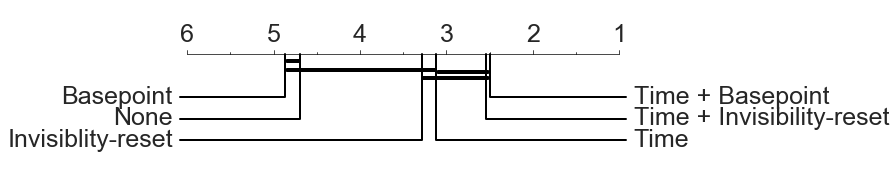
\includegraphics[width=0.5\linewidth]{images/basic_augs.png}
  		\caption{Performance of invariance-removing augmentations.}
  		\label{fig:basic_augs}
	\end{figure}
	
	We see that augmenting with time, and either basepoint or invisibility-reset, are both typically important. This is expected; in general a problem need not be invariant to either translation or reparametersiation.
	
	The second category consists of those augmentations which either seek to reduce dimensionality or introduce additional information. See Figure \ref{fig:all_augs}.
	
	\begin{figure}[h]
	  	\centering
	  	\vspace{-1em}
  		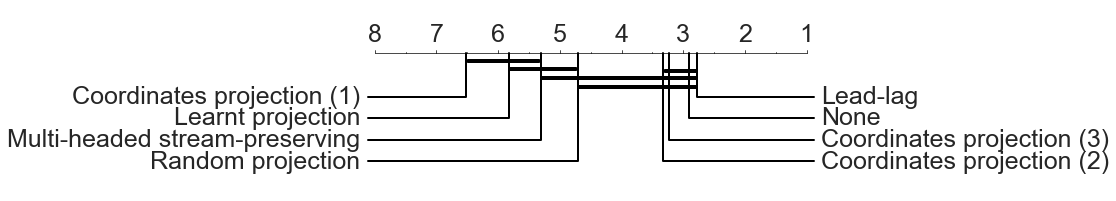
\includegraphics[width=0.65\linewidth]{images/all_augs.png}
  		\caption{Performance of other augmentations.}
  		\label{fig:all_augs}
	\end{figure}
	
	We see that most augmentations actually do not help matters, except for lead-lag which usually represents a good choice. We posit that the best augmentation is likely to be dataset dependent, so we additionally break this down by dataset characteristics in Table \ref{tab:augs_ranks_by_type}.

	\begin{table}[t]
	\centering
	\caption{Average ranks for different augmentations by dataset characteristics. Lower is better.}
	\label{tab:augs_ranks_by_type}
	\begin{tabular}{lcccccccc}
	\toprule
	& \multicolumn{8}{c}{\textbf{Augmentation}}\\
	 \cmidrule{2-9}
	 \multirow{2}{*}{\textbf{Characteristic}}&\multirow{2}{*}{None}& \multirow{2}{*}{Lead-lag}& \multicolumn{3}{c}{Coordinates projection} & Random& Learnt &  \multirow{2}{*}{MHSP}    \\
	 & & & (1) & (2) &(3) & projection &  projection \\
	\midrule
	\textbf{Data type} \\
	\cmidrule{1-1}
	EEG & 4.88 & 4.83 & 6.50 & 3.13 & 5.67 & 4.38 & \textbf{2.75} & \textbf{2.75} \\
	HAR & 2.25 & \textbf{1.78} & 7.20 & 3.50 & 2.90 & 4.75 & 6.50 & 6.50 \\
	MOTION & 2.63 & \textbf{1.75} & 7.00 & 4.50 & 2.13 & 5.00 & 7.33 & 5.00 \\
	OTHER & 2.88 & 3.92 & 5.44 & \textbf{2.63} & 3.29 & 4.69 & 6.00 & 5.21 \\
	\midrule
	\textbf{Series length}\\
	\cmidrule{1-1}
	$<$50 & 3.20 & \textbf{2.20} & 7.40 & 3.20 & 2.70 & 5.10 & 7.00 & 5.20 \\
	50-100 & 2.20 & \textbf{1.33} & 6.00 & 4.10 & 2.75 & 6.20 & 4.80 & 5.10 \\
	100-500 & \textbf{2.28} & 2.57 & 7.28 & 3.50 & 2.63 & 4.17 & 6.63 & 5.33 \\
	$>$500 & 4.00 & 4.00 & 5.28 & \textbf{2.64} & 4.57 & 4.07 & 4.40 & 5.60 \\
	\midrule
	\textbf{Dimension $d$}\\
	\cmidrule{1-1}
	2 & 4.67 & 3.5 & 6.33 & 4.33 & 4.0 & \textbf{2.83} & 6.67 & 3.67 \\
	3-5 & 2.5 & \textbf{2.21} & 6.36 & 3.43 & 3.14 & 4.64 & 6.67 & 6.83 \\
	6-8 & 3.25 & \textbf{2.5} & 6.94 & 3.0 & 3.56 & 5.0 & 5.29 & 6.0 \\
	$>$8 & \textbf{2.25} & 3.75 & 6.31 & 3.19 & 2.5 & 5.19 & 5.29 & 4.19\\
	\bottomrule           
	\end{tabular}
	\end{table}

	Here we indeed see that there is generally a better choice than doing nothing at all, but that this better choice is dependent on some characteristic of the dataset. For example on long or high-dimensional datasets, coordinate projections often perform well, whilst multi-headed stream preserving transformations do substantially better on EEG datasets. Lead-lag remains a strong choice in many cases.
	
	\paragraph{Windows} We consider the possibility of global, sliding, expanding, and dyadic windows. The results are shown in Figure \ref{fig:window}.
	
	\begin{figure}[h]
  		\centering
	  	\vspace{-1em}
  		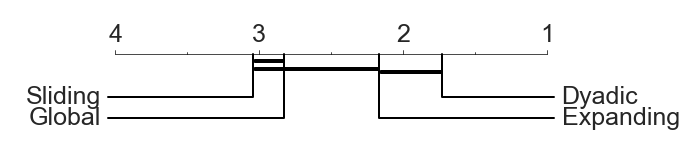
\includegraphics[width=0.45\linewidth]{images/window.png}
  		\caption{Performance of different windows.}
  		\label{fig:window}
	\end{figure}
	
	We see that the dyadic window is significantly better than sliding and global windows. The poor performance of sliding windows is a little surprising, but tallies with the observations of \citet{fermanian2019embedding}. This is an important finding, as global and sliding windows tend to be commonly used with signature methods.

	\paragraph{Signature versus logsignature transforms} We consider the signature and logsignature transforms with depths ranging from 1 to 6. As higher depths always produce more information, we define the performance of the (log)signature transform as the best performance across all depths. With this metric, the average rank of the signature transform was 1.23 whilst the average rank of the logsignature transform was 1.77, corresponding to a p-value of 0.01 with the Wilcoxon signed-rank test. Thus we find that the signature transform performs significantly better than the logsignature transform.

	\paragraph{Rescaling} We consider using no rescaling, pre-signature rescaling, or post-signature rescaling. See Figure \ref{fig:rescaling}. We see that pre-signature rescaling performs significantly worse than the other two options.
	
	\begin{figure}[h]
  		\centering
	  	\vspace{-1em}
  		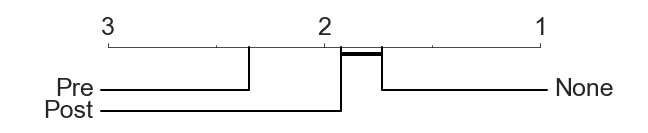
\includegraphics[width=.45\linewidth]{images/rescaling.png}
  		\caption{Performance of different rescalings}
  		\label{fig:rescaling}
	\end{figure}

	\subsection{A canonical signature method}
	\label{sec:performance}

	Given the results in the previous section, we derive a simple canonical signature method.
	\begin{enumerate}
		\item Unless the problem is known to be translation or reparameterisation invariant, then use the time and basepoint augmentations. Basepoint and invisbility-reset produce essentially the same performance, so basepoint is recommended over invisibility-reset due to its lower computational cost, as it does not introduce an extra channel.
		\item The lead-lag augmentation should be considered, but we do not recommend it in general. This is because the performance improvement it offers is relatively slight, and it is an expensive augmentation, due to its doubling of the number of pre-signature channels; recall that the number of signature features scales according to $\bigO(d^N)$, where $d$ is the input channels and $N$ is the depth of the (log)signature.
		\item Use hierarchical dyadic windows, and the signature transform; both have a depth hyperparameter that must be optimised.
	\end{enumerate}
	We emphasise that this does not represent a best option for every application, but is meant to represent a compromise between broad applicability, ease of implementation, computational cost, and good performance. To validate that these choices work well collectively, we investigate its performance on all 30 datasets from the UEA archive.

	Figure \ref{fig:best_rf} shows the critical difference plot of the canonical signature pipeline, combined with a random forest, against the benchmark classifiers of \citet{bagnall2018uea}, which are nearest-neighbours with either Euclidean (ED) or dynamic time warping (DTW) based distances. These have been shown by \citet{bagnall2017great} to represent a strong baseline for domain-independent time series classification.
	
	\begin{figure}[h]
  		\centering
	  	\vspace{-1em}
  		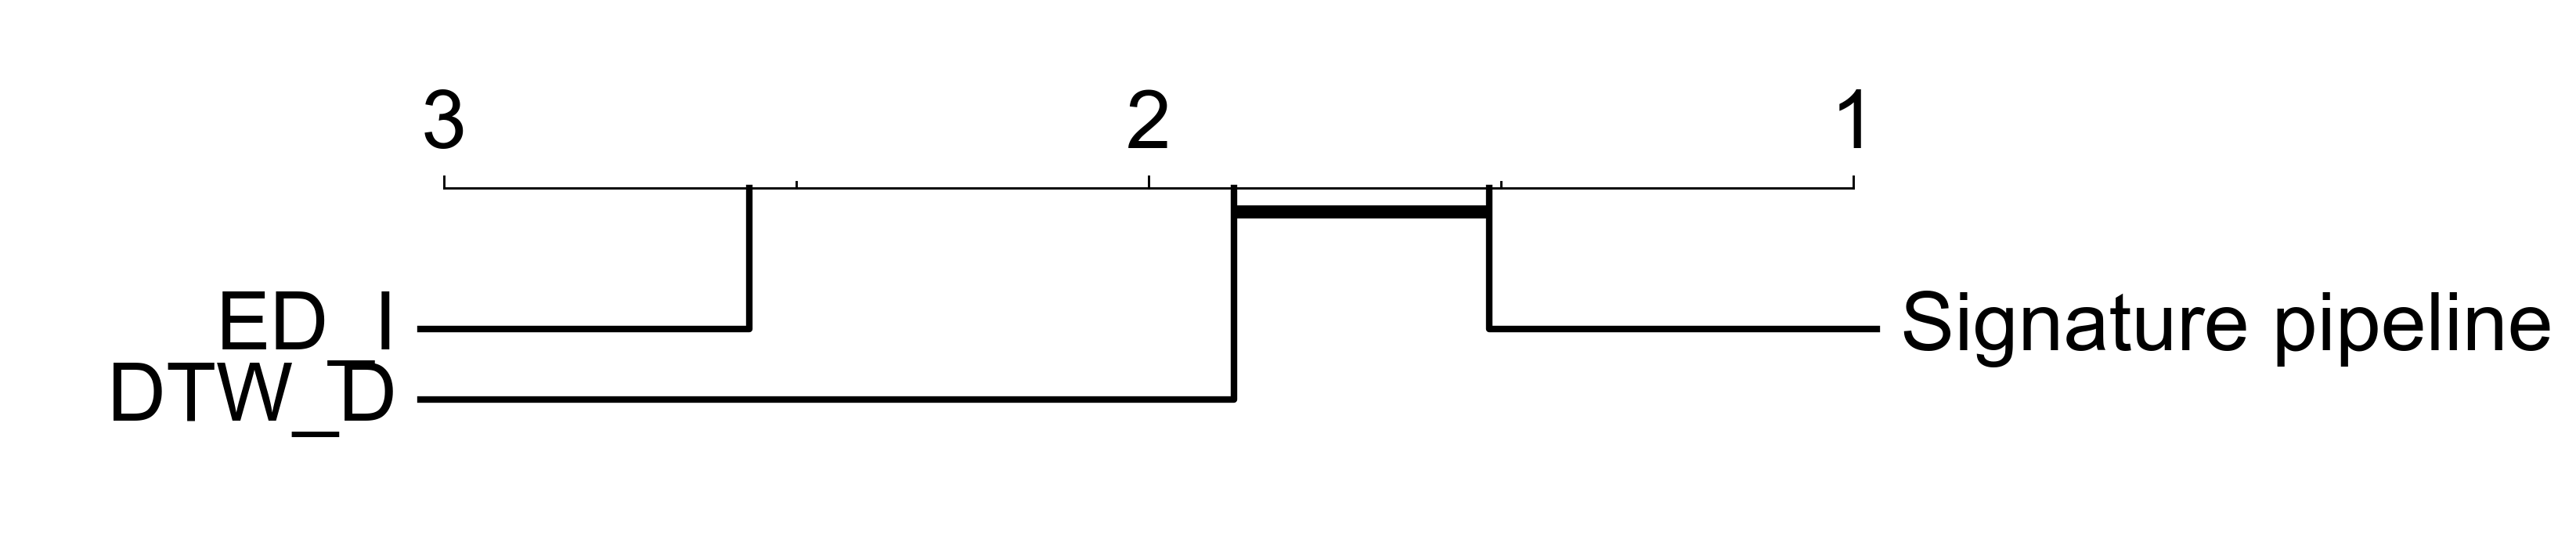
\includegraphics[width=.45\linewidth]{images/bestsig_wilcoxon.png}
  		\caption{Performance on UEA datasets.}
  		\label{fig:best_rf}
	\end{figure}
	
	 We see that our canonical signature method is significantly better than the previous benchmarks. Further comparisons to other benchmarks are beyond the scope of this paper; our primary goal is to compare the variations of the signature method against each other, and we refer to the existing literature for comparisons of the signature method against other methods. % CITE: TODO
	
	See Appendix \ref{sec:best_rf_details} for further details.
	
	\subsection{Further results}
	See Appendix \ref{sec:additional_results} for further results, in particular on the running times, sensitivity-inducing augmentations broken down by dataset type, an additional study on the most effective depth for the signature, and the precise numerical results for each individual test considered here.

	\section{Conclusion}
	We introduce a generalised signature method as a framework to capture recently proposed variations on the signature method. In doing so we are able to understand their conceptual groupings, and thus also understand how different variations may be combined. We go on to perform a first-of-its-kind extensive empirical investigation across 26 datasets, as to which elements of this framework are most important for performance in a domain-independent setting. As a result, we are able to present a canonical signature method that represents a best-practices domain-agnostic starting point, which may be fine tuned to any particular task.

	\section*{Broader impact}
	Many variations have been proposed on the signature method, and so we hope that the present paper will be of benefit to the signature community, through its introduction of a common language for the method and introduction of a canonical domain-independent signature method. As signatures are a subset of the time series analysis community, we expect to indirectly be of benefit to the broader community as well. We do not expect any specific negative outcomes from the broader impact of this paper.
	
	\section*{Acknowledgements}
	Thanks to Tony Bagnall for putting together the UEA datasets that were used in this paper. AF thanks G{\'e}rard Biau for stimulating discussions and insightful suggestions. JM was supported by the EPSRC grant EP/L015803/1 in collaboration with Iterex Therapuetics. AF was supported by a grant from R{\'e}gion Ile-de-France. PK was supported by the EPSRC grant EP/L015811/1. JM, PK, TL were supported by the Alan Turing Institute under the EPSRC grant EP/N510129/1.

	 


	\small
	\bibliography{references} 
	\bibliographystyle{apalike}
	\normalsize
	\newpage
	\appendix
	\begin{center}
	\huge Supplementary material
	\end{center}

	\section{Augmentations}
	\label{sec:augmentations_details}

	We recall that an augmentation is a map
	\begin{align*}
	\phi \colon  \tseries{\reals^d} &\to \tseries{\reals^e}^p
	\end{align*}
	We give below the precise definition of the different augmentations considered in the study, which are summarized in Table \ref{tab:summary_augmentations}. These augmentations were not typically introduced using such language, so this serves as a reference for how the existing literature may be interpreted through the generalised signature method.	
	
	Throughout the section, we consider a sequence $\mathbf{x}=(x_1,\dots,x_n) \in \tseries{\reals^d}$.

		\begin{table}[h]
	\centering
	\caption{Summary of the different augmentations}
	\label{tab:summary_augmentations}
	\begin{tabular}{llll l}
	\toprule
	 & $e$ & $p$ & Property  \\
	\midrule
	\multicolumn{4}{l}{Fixed augmentations} \\
	\cmidrule(r){1-1}
	None                                & $d$   & 1     &      \\
	Time                                & $d+1$ & 1     & sensitivity to parametrization, \\
										&		&		& uniqueness of the signature map \\
	Invisibility-reset                  & $d+1$ & 1     & sensitivity to translation  \\
	Basepoint                           & $d$   & 1     & sensitivity to translation  \\
	Lead-lag   	                        & $2d$  & 1     & information about quadratic variation, \\
										&		&		& uniqueness of the signature map \\
	Coordinates projection &     &   & dimensionality reduction \\
	\qquad with singletons & 1 & $d$ & \\
	\qquad with pairs  & 2     & $d(d-1)$ &  \\
	\qquad with triplets  & 3     & $d(d^2-1)$&\\
	Random projections                  & $e$   & $p$     & dimensionality reduction \\
	\cmidrule(r){1-1}
	\multicolumn{4}{l}{Learnt augmentations} \\
	\cmidrule(r){1-1}
	Learnt projections 	& $e$	& $p$		& data-dependent and linear \\
	Stream-preserving neural network & $e$ & $1$ & data-dependent \\
	Multi-headed stream-preserving NN      & $e$   & $p$   &  data-dependent  \\
	\bottomrule
	\end{tabular}
	\end{table}

	\paragraph{Time augmentation}
	
%		The time-joined transform of \citet{levin2013learning} or time-augmented path of \citet[Definition A.3]{kidger2019deep} is then
%	\begin{equation*}
%	\phi_{\mathbf{t}}(\mathb{x}) = ((t_1, x_1), \ldots, (t_n, x_n)) \in \tseries(\reals^{d + 1}),
%	\end{equation*}
%	which ensures that the signature is sensitive to changes in speed.

	For a regularly sampled time series, the time augmentation is defined by
	\begin{equation*}
	\phi(\mathbf{x})= \big((1,x_1),\dots,(n,x_n) \big) \in \tseries{\reals^{d+1}}.
	\end{equation*}
	It ensures uniqueness of the signature transformation and removes the parametrization invariance \citep{levin2013learning}.
	
	If the time series is irregularly sampled, and there is an additional sequence of timestamps $\mathbf{t} = (t_1, \ldots, t_n) \in \tseries{\reals}$ such that $\len{\mathbf{t}} = \len{\mathbf{x}}$, then this is instead defined as
	\begin{equation*}
	\phi_{\mathbf{t}}(\mathbf{x})= \big((t_1,x_1),\dots,(t_n,x_n) \big) \in \tseries{\reals^{d+1}}.
	\end{equation*}

	\paragraph{Invisibility-reset augmentation}

	First introduced by \citet{yang2017leveraging}, the invisibility-reset augmentation consists in adding a coordinate to the sequence $\mathbf{x}$ that is constant equal to 1 but drops to 0 at the last time step, i.e.,
	\begin{equation*}
	\phi(\mathbf{x})= \big((1,x_1),\dots,(1,x_{n-1}) ,(1,x_n),(0,x_n),(0,0) \big) \in \tseries{\reals^{d+1}}.
	\end{equation*}
	This augmentation adds information on the initial position of the path, which is otherwise not included in the signature as it is a translation-invariant map.

	\paragraph{Basepoint augmentation}
	Introduced by \citet{signatory}, the basepoint augmentation has the same goal as the invisibility-reset augmentation: removing the translation-invariant property of the signature. It simply adds the point 0 at the beginning of the sequence:
	\begin{equation*}
	\phi(\mathbf{x})= (0,x_1,\dots,x_n) \in \tseries{\reals^{d}}.
	\end{equation*}
	The main difference compared to the invisibility-reset augmentation is that the signature of $\mathbf{x}$ is contained in the signature of the invisibility-reset augmented path, whereas it is not in the signature of the basepoint augmented path. The price paid is that the invisibility-reset augmentation introduces redundancy into the signature, and is more computationally expensive due to the additional channel. (Recall that the signature method scales as $\bigO(d^N)$, where $d$ is the input channels and $N$ is the depth of the (log)signature.)

	\paragraph{Lead-lag augmentation}

	The lead-lag augmentation, introduced by \citet{primer2016} and \citet{flint2016discretely} has been used in several applications (See for example \citet{lyons2014feature,kormilitzin2016application,yang2017leveraging}). It adds lagged copies of the path as new coordinates. This then explicitly captures the quadratic variation of the underlying process \citep{flint2016discretely}. As many different lags as desired may be added. If there is a single lag of a single timestep, then this corresponds to
	\begin{equation*}
	\phi(\mathbf{x})= ((x_1,x_1),(x_2,x_1),(x_2,x_2),\dots,(x_n,x_n)) \in \tseries{\reals^{2d}}.
	\end{equation*}
	
	\paragraph{Coordinate projections}
	For multidimensional streams, one may want to compute the signature of a subset of coordinates individually, rather than the signature of the whole stream; doing so restricts the interaction considered by the signature to just those between the projected coordinates. Let $\mathbf{x^1},\dots, \mathbf{x^d} \in \tseries{\reals}$ denote the different coordinates of $\mathbf{x}\in \tseries{\reals^d}$. Let $\mathbf{t} = (1, \ldots, n) \in \tseries{\reals}$.
	
	Then we define the singleton coordinate projection as
	\begin{equation*}
	\phi(\mathbf{x})= \big((\mathbf{t},\mathbf{x^1}),(\mathbf{t},\mathbf{x^2}),\dots,(\mathbf{t},\mathbf{x^{d}}) \in \tseries{\reals^2}^{d},
	\end{equation*}
	whilst considering all possible pairs of coordinates yields the augmentation
	\begin{equation*}
	\phi(\mathbf{x})= \big((\mathbf{t}, \mathbf{x^1},\mathbf{x^2}),(\mathbf{t}, \mathbf{x^1},\mathbf{x^3}),\dots,(\mathbf{t}, \mathbf{x^d},\mathbf{x^{d-1}}) \in \tseries{\reals^2}^{d(d-1)},
	\end{equation*}
	and all possible triples yields the augmentation
	\begin{equation*}
	\phi(\mathbf{x})= \big((\mathbf{t}, \mathbf{x^1},\mathbf{x^1},\mathbf{x^2}),(\mathbf{t}, \mathbf{x^1},\mathbf{x^1},\mathbf{x^3}),\dots,(\mathbf{t}, \mathbf{x^{d}},\mathbf{x^d},\mathbf{x^{d-1}}) \in \tseries{\reals^3}^{d(d^2-1)}.
	\end{equation*}
	
	The decision to always include a time dimension is a somewhat arbitrary one, and it may alternatively be excluded if desired. (This is done so as to make sense of singleton coordinate projections; otherwise the result is a collection of univariate time series, for which the signature extracts only the increment due to the tree-like equivalence property.)
	
	\paragraph{Random projections}
	When the dimension of the input path is very large, \citet{lyons2017sketching} have proposed to project it into a smaller space by taking multiple random projections. Let $e<d$ and let $A_i:\reals^d \to \reals^{e}$ be random affine transformations indexed by $i \in \{1, \ldots, p\}$. Then $\phi$ is defined as
	\begin{equation*}
	\phi(\mathbf{x})= ((A_1 x_1,\dots,A_1 x_n), \ldots, (A_p x_1,\dots,A_p x_n)) \in \tseries{\reals^{e}}^p.
	\end{equation*}
	
	\paragraph{Learnt projections}
	Rather than taking random projections, \citet{logsig-rnn} learn it from the data. This takes exactly the same form as the random projections, except that the $A_i$ are learnt.
	
	\paragraph{Stream-preserving neural network}
	\citet{kidger2019deep} introduce arbitrary learnt sequence-to-sequences maps prior to the signature transform, and refer to such maps, when parameterised as neural networks, as stream-preserving neural networks. For example these may be standard convolutional or recurrent architectures. In general this may be any learnt transformation
	\begin{equation*}
	\phi \colon \tseries{\reals^d} \to \tseries{\reals^e}.
	\end{equation*}

	\paragraph{Multi-headed stream-preserving neural network}
	A straightforward extension of stream-preserving neural networks is to use multiple such networks, so as to avoid a potential bottleneck through the single signature map that it is eventually used in. Letting $\phi^1, \ldots, \phi^p$ be $p$ different stream-preserving neural networks, then this gives an augmentation
	\begin{equation*}
	\phi(\mathbf{x}) = (\phi^1(\mathbf{x}), \ldots, \phi^p(\mathbf{x})) \in (\tseries{\reals^e})^p.
	\end{equation*}

	\section{Implementation details}
	\label{sec:implementation_details}
	
	\subsection{General notes}
	
	\paragraph{Code} All the code for this project is available at\\ \texttt{https://github.com/jambo6/generalised-signature-method}.
	
	\paragraph{Libraries} The machine learning framework used was PyTorch \citep{pytorch} version 1.3.1. Signatures and logsignatures were computed using the Signatory library \citep{signatory} version 1.1.6. Scikit-learn \citep{scikit-learn} version 0.22.1 was used for the logistic regression and random forest models. The experiments were tracked using the Sacred framework \citep{greff2017sacred} version 0.8.1.

	\paragraph{Normalisation} Every dataset was normalised so that each channel has mean zero and unit variance.
	
	\paragraph{Architectures} Two different GRU models were used on every dataset; a `small' one with 32 hidden channels and 2 layers, and a `large' one with 256 hidden channels and 3 layers.
	
	Likewise, two different Residual CNN models were considered. The `small' one used 6 blocks, each composed of batch normalisation, ReLU activation, convolution with 32 filters and kernel size 4, batch normalisation, ReLU activation, and a final convolution with 32 filters and kernel size 4, so that there are also 32 channels along the `residual path'. A final two-hidden-layer neural network with 256 neurons was placed on the output. The `large' is similar, except that it used 128 filters in both the blocks and the residual path, had 8 blocks, used a kernel size of 8, and the final neural network had 1024 neurons.
	
	The logistic regression was performed three times with different amounts of $L^2$ regularisation, with scaling hyperparameters of 0.01, 0.2 and 1; for every experiment the regularization hyperparameter achieving the best accuracy on the test set was used.
	
	The random forest used the default Scikit-learn implementation with a maximum depth of 6 and 100 trees.
	
	\paragraph{Optimiser}The GRU and CNN were optimised using Adam \citep{adam}. The learning rate was 0.01 for the GRU, and 0.001 for the residual CNN. The small models were trained for a maximum of 500 epochs; the large models were trained for a maximum of 1000 epochs. The learning rate was decreased by a factor of 10 if validation loss did not improve over a plateau of 10 epochs. Early stopping was used if the validation loss did not improve for 30 epochs. After training the parameters were always rolled back to those that demonstrated the best validation loss over the course of training. The batch size used varied by dataset; in each it was taken to be the power of two that meant that the number of batches per epoch was closest to 40.
	
	\paragraph{Computing infrastructure}Experiments were run on an Amazon AWS G3 Instance (g3.16xlarge) equipped with 4 Tesla M60s, parallelized using GNUParallel \citep{Tange2011a}.

	\subsection{Analysis of variations of the signature method}\label{sec:omitted_experiments}\label{sec:experiment_details}
	\paragraph{Splits}
	The UEA archive comes with a pre-defined train-test split, which we respect. We take an 80\%/20\% train/validation split in the training data, stratified by class label. For the Human Activities and Postural Transitions dataset, we take a 60\%/15\%/25\% train/validation/test split from the whole dataset. For the Speech Commands dataset, we take a 68\%/17\%/15\% train/validation/test split from the whole dataset. (These somewhat odd choices corresponding to taking either 25\% or 15\% of the dataset as test, and then splitting the remaining 80\%/20\% between train and validation.) These train/validation splits are only used for the training of the GRU and CNN classifiers.
	
	\paragraph{Combinations}
	In total we tested 8569 different combinations.
	
	The variations tested are divided into groups. The first group consists of the sensitivity-adding augmentations, namely time, basepoint and invisibility-reset. Relative to the baseline model, we test every possible combination of these. (Including using none of them.)
	
	The second group consists of those other augmentations, namely the lead-lag, singleton coordinate projection, pair coordinate projection, triplet coordinate projection, random projections, learnt projections, and multi-headed stream preserving neural networks, and finally also the case of no additional augmentation.
	
	For the random projections, we consider four possibilities, with $e \in \{3, 6\}$ and $p \in \{2, 5\}$, all relative to the baseline model.
	
	For no additional augmentation, lead-lag, coordinate projections, learnt projections, and the multi-headed stream preserving neural networks, we compose them with the time, time+basepoint and time+invisibility-reset augmentations (the clear best three from the first group), all relative to the baseline model.
	
	For the learnt projections, we consider four different possibilities corresponding to $e \in \{3, 6\}$ and $p \in \{2, 5\}$; together with the time/time+basepoint/time+invisibility-reset cases this yields a total of twelve possibilities.
	
	For the multi-headed stream-preserving neural networks, we again consider four different possibilities corresponding to $e \in \{3, 6\}$ and $p \in \{2, 5\}$, for a total of twelve possible augmentation strategies. In each the neural network operates elementwise, so as to map one sequence to another, and is given by a feedforward neural network of three hidden layers separated by ReLU activation functions. When $e = 3$ the hidden layers have 16 neurons each, and when $e = 6$ they have 32 neurons each.
	
	For both the learnt projections and multi-headed stream-preserving neural networks, training these requires backpropagating through the model, so these were only considered for the GRU and residual CNN model. (The logistic regression model would in principle be possible as well, except that we ended up implementing this through Scikit-learn rather than PyTorch.)
	
	We note that there are a great many possible ways of doing stream preserving neural networks, of which these are a small fraction. Their relatively weak performance here may likely be improved upon with greater tuning on an individual task, or the selection of better final models than were considered here.
	
	The third group consisted of the different windows. Recall that the baseline model used a global window; we then consider varying this to two possible sliding windows, two possible expanding windows, and three possible dyadic windows. The two possible sliding/expanding windows are chosen so that either 5 or 20 windows are applied across the full length of the dataset. The three possible dyadic windows are depths 2, 3, 4. Thus in total there are 8 possible window combinations we consider.
	
	The fourth group consists of rescaling options, namely no rescaling, pre-signature rescaling, and post-signature rescaling.
	
	\paragraph{Omissions}
	For the empirical study on the variations on the signature method, we excluded those UEA datasets with a dimension $d$ over 60, so as to reduce the computational cost. This results removes 6 of the 30 datasets from the study, namely DuckDuckGeese, FaceDetection, Heartbeat, InsectWingbeat, MotorImagery, and PEMS-SF. These were nonetheless used in the demonstration of performance of the canonical signature method in Figure \ref{fig:best_rf}. Furthermore those combinations of dataset/variation/model which produced more than $10^5$ signature features were omitted, to keep the computation managable. See Table \ref{tab:omissions}.

	\begin{table}[h]
		\caption{Summary of the number of combinations considered and omitted.}\label{tab:omissions}
		\begin{tabular}{lcccc}
		\toprule
		\textbf{Variations } & \textbf{\# Variations} & \textbf{\# Classifiers} & \textbf{\# Omitted } &\textbf{\# Total}  \\
		& & & \textbf{Combinations} & \textbf{Combinations} \\
		\midrule
		Basic augmentations (Figure \ref{fig:basic_augs}) & $6$ & $6$ & $54$ &  $936$\\
		\cmidrule{1-1}
		Other augmentations (Figure \ref{fig:all_augs}) \\
		Lead-lag/ None & $3$ & $6$ & $100$/$27$ & $468$ \\
		Coordinates projection (1)/(2)/(3)& $3$ & $6$ & $12$/$12$/$54$ & $468$ \\
		Random projections & $4$ & $6$ & $32$ & $624$ \\
		Learnt projections / MHSP & $12$ & $4$ & $348$/$176$ & $1248$\\
		\cmidrule{1-1}
		Windows (Figure \ref{fig:window}) & $8$ & $6$ & $227$ & $1248$ \\
		\cmidrule{1-1}
		Signature/Logsignature transform & $12$ & $6$ &$361$ &$1872$ \\ 
		\cmidrule{1-1}
		Rescalings (Figure \ref{fig:rescaling}) & $3$ & $6$ &$12$ & $468$ \\
		\midrule{}
		\textbf{Total} & & & $1415$ & $9984$ \\
		\bottomrule
		\end{tabular}
	\end{table}
	

	\subsection{The canonical signature pipeline}
	\label{sec:best_rf_details}

	For each dataset, we implement the following steps. First, the sequences are augmented with time and basepoint augmentations. Then, we consider every combination of signature depth in $\{1, 2, 3, 4, 5, 6\}$ and hierarchical dyadic window depth in $\{2, 3, 4\}$. We consider `post' rescaling of the signature features. For each of these choices, we perform a randomized grid search on a random forest classifier to optimize its number of trees and maximal depth parameters. We test 20 combinations randomly sampled from the following grids:
	\begin{align*}
	    \textnormal{n\_trees}&=[50, 100, 500, 1000], \\
       \textnormal{max\_depth}&=[2, 4, 6, 8, 12, 16, 24, 32, 45, 60, 80, \textnormal{None}].
     \end{align*}
     Note that a maximal depth set to `None' means that the trees are expanded until all leaves contain exactly one sample. Finally, we choose the combination of signature and hierarchical dyadic window depths which maximise the out-of-bag score. 
     
     	\section{Additional results}
	\label{sec:additional_results}

	\subsection{Analysis of variations of the signature method}
	\paragraph{Running time}
	To get a sense of the cost of each augmentation or window, we present the run times of each augmentation/model combination, and each window/model combination. (The times for varying between signature and logsignature, and between different rescalings, are largely insignificant.) See Table \ref{tab:average_run_time}.
	
	The run times are averaged over every UEA dataset. As the datasets are of very different sizes this thus represents quite a crude statistic, and in particular produces very large variances, so these are most meaningful simply with respect to each other.
	
	\begin{table}[h]
		\caption{Average run time (in seconds) for various experiments. mean (std), averaged over all UEA datasets.}
		\label{tab:average_run_time}
		\begin{tabular}{lcccc}
		\toprule
		&\multicolumn{4}{c}{\textbf{Classifier}} \\
		\cmidrule{2-5}
		 & \multirow{2}{*}{CNN} & \multirow{2}{*}{GRU} & Logistic  & Random \\
		 & & & regression & forest \\
		\midrule
		%Average over all experiments &369 (965) & 429 (1996) &  \textbf{4.34 (14.2)} &  22.3 (155)\\
		%\midrule
		\parbox{51mm}{Time augmentation+Global window\\(Baseline)} & 69.8 (98.0) & 22.2 (31.8) & 2.67 (7.09) & 2.23 (4.84) \\
		\midrule
		\textbf{Augmentation} & & & \\
		\cmidrule{1-1}
		None & 48.1 (63.5) & 16.8 (33.6) & 3.55 (9.91) & 66.3 (321) \\
		Lead-lag & 48.58 (69.99) & 15.2 (18.1) & 5.76 (11.7) & 3.35 (6.04) \\
		Coordinates projection (1) & 32.8 (31.49) & {13.4 (17.8) }& 1.37 (4.2) & 12.2 (59.3) \\
		Coordinates projection (2) & 41.5 (51.4) & 22.6 (62.3) & 3.01 (8.54) & 42.3 (203) \\
		Coordinates projection (3) & {41.3 (39.9)} & 19.1 (24.5) & 5.41 (9.76) & 6.3 (14.1) \\
		Random projection & 62.2 (70.1) & 21.1 (31.2) & {0.86 (1.25) }& {1.4 (2.47) }\\
		Learnt projection & 917 (1288) & 752 (972) & -- & -- \\
		Multi-headed stream-preserving & 1051 (1677) & 1758 (4442) & -- & -- \\
		\cmidrule{1-1}
		\textbf{Window}  & & & \\
		\cmidrule{1-1}
		Sliding & 90.6 (120) & 79.4 (175) & 10.1 (27.4) & 6.4 (16.0) \\
		Expanding & 102 (133) & 68.7 (115) & 9.98 (27.2) & 7.17 (19.0) \\
		Dyadic & 725 (868) & 56.9 (65.1) & 12.5 (33.2) & 7.59 (18.3) \\
		\bottomrule
		\end{tabular}
		\end{table}

	\paragraph{Sensitivity-inducing augmentations broken down by dataset type}

	Table \ref{tab:basic_augs_ranks_by_type} shows the average rank of each of the first group of augmentations (that add sensitivity to certain kinds of perturbation) by dataset type, where the types are taken from \citet{bagnall2018uea}. (This may be regarded as a companion to Table \ref{tab:augs_ranks_by_type}.)
	
	It is interesting to note that for EEG data, it seems better not to consider the time augmentation, whereas it is the case for other applications. In particular the combination of time and basepoint augmentations achieve the best ranks for human action and motion recognition (HAR and MOTION in Table \ref{tab:basic_augs_ranks_by_type}). Recognizing an action may not be translation-invariant nor invariant by time reparametrization.
	
	\begin{table}[h]
	\caption{Average ranks for different augmentations by type of data. Lower is better.}
	\label{tab:basic_augs_ranks_by_type}
	\centering
		\begin{tabular}{lllllll}
		\toprule
	 & \multicolumn{6}{c}{\textbf{Augmentation}}\\
	 \cmidrule{2-7}
	\multirow{2}{*}{\textbf{Data type}} &\multirow{2}{*}{None } &\multirow{2}{*}{Time} &\multirow{2}{*}{Basepoint}& \multirow{2}{*}{Invisibility-reset}    & Time + & Time +        \\
		& & & & & Basepoint & Invisibility-reset  \\
		\midrule
		EEG & 3.88 & 3.50 & 4.00 & \textbf{2.00} & 4.00 & 3.63 \\
		HAR & 5.00 & 2.95 & 4.85 & 3.65 & \textbf{2.00} & 2.55 \\
		MOTION & 5.25 & 2.75 & 5.75 & 3.88 & \textbf{1.50} & 1.88 \\
		OTHER & 4.43 & 3.31 & 4.88 & 3.19 & 2.87 & \textbf{2.31 } \\ 
		\bottomrule
		\end{tabular}
	\end{table}


	\paragraph{Depth study on the signature transform}
	In the main text we focused on the difference between the signature and logsignature transforms, and stated that larger depths must be chosen by a bias-variance tradeoff. Here we consider varying the depth together with the choice of signature or logsignature, and taking the best transform for each depth. See Figure \ref{fig:depth}. We see that larger depths do indeed generally correspond to increased performance, up to a point. The optimal depth will depend on the complexity of the task, as the number of features increases exponentially with the depth.
	
	\begin{figure}[h]
  		\centering
  		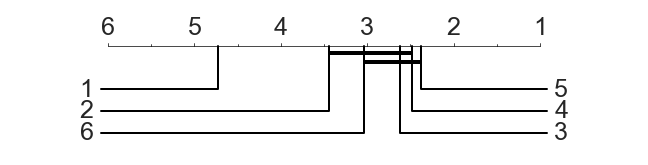
\includegraphics[width=.6\linewidth]{images/depth.png}
  		\caption{Critical differences plot for the depth study on the UEA datasets.}
  		\label{fig:depth}
	\end{figure}

	\subsection{Complete results}

	We present in Tables \ref{tab:complete_results_basic_augs}, \ref{tab:complete_results_all_augs}, \ref{tab:complete_results_windows}, \ref{tab:complete_results_sig_logsig}, \ref{tab:complete_results_rescaling} and \ref{tab:complete_results_depth} the performance of the different signature variations on each dataset. The tables were obtained by maximizing the test accuracy of the signature method over the different classifiers considered. Recall that some values are omitted due to the large number of signature features that would be obtained.


	\begin{table}[h]
	\small
	\centering
	\caption{Accuracy of sensitivity-inducing augmentations per dataset}
	\label{tab:complete_results_basic_augs}
	\begin{tabular}{lcccccc}
	\toprule
	 & \multicolumn{6}{c}{\textbf{Augmentation}}\\
	 \cmidrule{2-7}
	\multirow{2}{*}{\textbf{Dataset}} &\multirow{2}{*}{None } &\multirow{2}{*}{Time} &\multirow{2}{*}{Basepoint}& \multirow{2}{*}{Invisibility-reset}    & Time + & Time +        \\
		& & & & & Basepoint & Invisibility-reset  \\
	\midrule
	ArticularyWordRecognition & 96.0\% & 96.3\% & 95.7\% & 96.3\% & 97.7\% & 97.0\% \\
	AtrialFibrillation & 46.7\% & 46.7\% & 40.0\% & 33.3\% & 40.0\% & 40.0\% \\
	BasicMotions & 100.0\% & 100.0\% & 100.0\% & 100.0\% & 100.0\% & 100.0\% \\
	CharacterTrajectories & 88.3\% & 93.2\% & 86.4\% & 88.7\% & 93.8\% & 93.7\% \\
	Cricket & 91.7\% & 94.4\% & 94.4\% & 97.2\% & 97.2\% & 95.8\% \\
	ERing & 80.0\% & 92.6\% & 77.4\% & 89.6\% & 91.9\% & 92.2\% \\
	EigenWorms & 72.5\% & 79.4\% & 74.8\% & 76.3\% & 87.0\% & 81.7\% \\
	Epilepsy & 84.8\% & 89.9\% & 91.3\% & 91.3\% & 97.1\% & 94.9\% \\
	EthanolConcentration & 27.8\% & 29.3\% & 33.5\% & 41.8\% & 34.6\% & 41.4\% \\
	FingerMovements & 55.0\% & 52.0\% & 57.0\% & 58.0\% & 55.0\% & 56.0\% \\
	HandMovementDirection & 29.7\% & 33.8\% & 32.4\% & 33.8\% & 36.5\% & 32.4\% \\
	Handwriting & 21.9\% & 30.8\% & 23.6\% & 24.6\% & 30.6\% & 28.7\% \\
	JapaneseVowels & 85.4\% & 85.1\% & 97.3\% & 98.1\% & 97.3\% & 98.1\% \\
	LSST & 42.0\% & 47.4\% & 44.0\% & 44.4\% & 50.9\% & 48.7\% \\
	Libras & 72.8\% & 84.4\% & 65.0\% & 75.0\% & 80.0\% & 77.2\% \\
	NATOPS & 81.7\% & 88.3\% & 79.4\% & 79.4\% & 91.1\% & 92.2\% \\
	PenDigits & 91.1\% & 97.1\% & 88.3\% & 93.1\% & 96.8\% & 97.1\% \\
	PhonemeSpectra & 4.7\% & 8.2\% & 4.3\% & 5.7\% & 10.0\% & 8.1\% \\
	RacketSports & 78.9\% & 80.3\% & 78.9\% & 82.9\% & 82.9\% & 81.6\% \\
	SelfRegulationSCP1 & 81.6\% & 83.3\% & 76.8\% & 84.0\% & 75.4\% & 85.0\% \\
	SelfRegulationSCP2 & 57.2\% & 56.7\% & 56.1\% & 56.7\% & 56.1\% & 55.0\% \\
	SpokenArabicDigits & 82.5\% & 85.5\% & 80.5\% & 88.0\% & 85.1\% & 90.1\% \\
	StandWalkJump & 60.0\% & 46.7\% & 40.0\% & 46.7\% & 40.0\% & 46.7\% \\
	UWaveGestureLibrary & 84.1\% & 87.5\% & 79.7\% & 82.8\% & 87.5\% & 83.4\% \\
	Human Activity & 73.0\% & 76.6\% & 92.3\% & 92.2\% & 93.0\% & 93.8\% \\
	Speech Commands & 71.4\% & 75.9\% & 74.7\% & 74.9\% & 79.7\% & 79.5\% \\
	\midrule
	Average rank &  4.69 & 3.12 & 4.87 & 3.29 & \textbf{2.5} & 2.54 \\
	\bottomrule
	\end{tabular}
	\end{table}



	\begin{table}[h]
	\small
	\centering
	\caption{Accuracy of other augmentations per dataset}
	\label{tab:complete_results_all_augs}
	\begin{tabular}{lcccccccc}
	\toprule
	& \multicolumn{8}{c}{\textbf{Augmentation}}\\
	 \cmidrule{2-9}
	 \multirow{2}{*}{\textbf{Dataset}}&\multirow{2}{*}{None}& \multirow{2}{*}{Lead-lag}& \multicolumn{3}{c}{Coordinates projection} & Random& Learnt &  \multirow{2}{*}{MHSP}    \\
	 & & & (1) & (2) &(3) & projection &  projection \\
	\midrule
	ArticularyWordRecognition & 97.7\% & 96.3\% & 83.3\% & 95.7\% & 97.0\% & 95.3\% & 73.7\% & 80.3\% \\
	AtrialFibrillation & 46.7\% & 40.0\% & 53.3\% & 53.3\% & 46.7\% & 66.7\% & 46.7\% & 53.3\% \\
	BasicMotions & 100.0\% & 100.0\% & 80.0\% & 100.0\% & 100.0\% & 100.0\% & 97.5\% & 87.5\% \\
	CharacterTrajectories & 93.8\% & 95.3\% & 43.9\% & 93.2\% & 93.8\% & 93.3\% & 89.6\% & 91.1\% \\
	Cricket & 97.2\% & 98.6\% & 90.3\% & 97.2\% & 95.8\% & 88.9\% & 69.4\% & 56.9\% \\
	ERing & 92.6\% & 94.8\% & 79.3\% & 89.3\% & 91.9\% & 74.4\% & 62.2\% & 61.1\% \\
	EigenWorms & 87.0\% & 87.8\% & 50.4\% & 84.0\% & 89.3\% & 78.6\% & -- & -- \\
	Epilepsy & 97.1\% & 97.1\% & 55.8\% & 95.7\% & 95.7\% & 81.9\% & 67.4\% & 65.9\% \\
	EthanolConcentration & 41.4\% & 39.9\% & 42.2\% & 43.3\% & 42.2\% & 30.4\% & 32.3\% & 30.0\% \\
	FingerMovements & 56.0\% & -- & 59.0\% & 58.0\% & -- & 55.0\% & 60.0\% & 65.0\% \\
	HandMovementDirection & 36.5\% & 31.1\% & 31.1\% & 40.5\% & 37.8\% & 37.8\% & 33.8\% & 44.6\% \\
	Handwriting & 30.8\% & 33.5\% & 11.3\% & 27.8\% & 30.0\% & 21.6\% & 12.6\% & 13.2\% \\
	JapaneseVowels & 98.1\% & 97.6\% & 94.1\% & 97.8\% & 97.6\% & 84.1\% & 95.4\% & 95.9\% \\
	LSST & 50.9\% & 55.6\% & 43.5\% & 51.7\% & 52.8\% & 43.7\% & 34.4\% & 39.8\% \\
	Libras & 84.4\% & 86.7\% & 47.8\% & 83.9\% & 85.0\% & 86.7\% & 73.3\% & 81.1\% \\
	NATOPS & 92.2\% & -- & 33.3\% & 90.6\% & 91.1\% & 85.6\% & 83.9\% & 81.7\% \\
	PenDigits & 97.1\% & 98.3\% & 60.2\% & 96.8\% & 97.2\% & 96.7\% & 96.5\% & 97.4\% \\
	PhonemeSpectra & 10.0\% & -- & 4.5\% & 9.4\% & 10.6\% & 8.9\% & 7.2\% & 7.7\% \\
	RacketSports & 82.9\% & 82.2\% & 53.3\% & 85.5\% & 84.2\% & 75.7\% & 73.7\% & 75.0\% \\
	SelfRegulationSCP1 & 85.0\% & 86.0\% & 61.8\% & 85.0\% & 84.0\% & 81.6\% & 86.7\% & 84.6\% \\
	SelfRegulationSCP2 & 56.7\% & 57.2\% & 55.6\% & 58.9\% & 55.6\% & 60.6\% & 59.4\% & 57.8\% \\
	SpokenArabicDigits & 90.1\% & 96.6\% & 58.5\% & 86.0\% & 90.0\% & 83.0\% & 88.0\% & 86.0\% \\
	StandWalkJump & 46.7\% & 40.0\% & 40.0\% & 53.3\% & 40.0\% & 53.3\% & -- & -- \\
	UWaveGestureLibrary & 87.5\% & 88.8\% & 50.6\% & 85.6\% & 87.5\% & 86.2\% & 74.1\% & 75.6\% \\
	Human Activity & 93.8\% & 93.6\% & 75.8\% & 93.2\% & 93.6\% & 69.2\% & 91.3\% & 91.5\% \\
	Speech Commands & 79.7\% & -- & 14.9\% & 77.1\% & -- & 70.2\% & -- & 76.1\% \\
	\midrule
	Average ranks & 2.9 & \textbf{2.77} & 6.52 & 3.33 & 3.23 & 4.71 & 5.83 & 5.31\\
	\bottomrule
	\end{tabular}
	\end{table}

	\begin{table}[h]
	\small
	\centering
	\caption{Accuracy of windows per dataset}
	\label{tab:complete_results_windows}
	\begin{tabular}{lcccc}
	\toprule
	& \multicolumn{4}{c}{\textbf{Window}}\\
	 \cmidrule{2-5}
	\textbf{Dataset}&Global & Sliding & Expanding & Dyadic  \\
	\midrule
	ArticularyWordRecognition & 96.3\% & 89.3\% & 99.0\% & 99.0\% \\
	AtrialFibrillation & 46.7\% & 46.7\% & 46.7\% & 60.0\% \\
	BasicMotions & 100.0\% & 100.0\% & 100.0\% & 100.0\% \\
	CharacterTrajectories & 93.2\% & 94.6\% & 96.9\% & 97.1\% \\
	Cricket & 97.2\% & 93.1\% & 97.2\% & 95.8\% \\
	ERing & 90.7\% & 88.5\% & 91.9\% & 94.8\% \\
	EigenWorms & 80.2\% & 74.8\% & 78.6\% & 76.3\% \\
	Epilepsy & 89.9\% & 92.8\% & 92.0\% & 94.2\% \\
	EthanolConcentration & 30.4\% & 38.8\% & 30.0\% & 35.7\% \\
	FingerMovements & 50.0\% & -- & -- & -- \\
	HandMovementDirection & 33.8\% & 33.8\% & 36.5\% & 33.8\% \\
	Handwriting & 30.1\% & 21.5\% & 30.2\% & 27.2\% \\
	JapaneseVowels & 85.1\% & 76.5\% & 88.1\% & 89.2\% \\
	LSST & 47.8\% & 43.1\% & 48.3\% & 46.6\% \\
	Libras & 83.3\% & 85.6\% & 91.1\% & 90.0\% \\
	NATOPS & 93.3\% & 84.4\% & 90.6\% & -- \\
	PenDigits & 95.8\% & -- & -- & 97.6\% \\
	PhonemeSpectra & 8.6\% & 9.2\% & 9.6\% & 10.4\% \\
	RacketSports & 82.2\% & 80.3\% & 84.2\% & 88.2\% \\
	SelfRegulationSCP1 & 82.6\% & 87.4\% & 84.0\% & 86.7\% \\
	SelfRegulationSCP2 & 56.7\% & 60.6\% & 54.4\% & 56.1\% \\
	SpokenArabicDigits & 85.5\% & 91.5\% & 93.7\% & 96.6\% \\
	StandWalkJump & 46.7\% & 53.3\% & 46.7\% & 53.3\% \\
	UWaveGestureLibrary & 86.6\% & 79.4\% & 89.1\% & 89.7\% \\
	Human Activity & 76.1\% & 73.0\% & 80.4\% & 81.7\% \\
	Speech Commands & 75.9\% & 76.5\% & 82.3\% & 83.0\% \\
	\midrule
	Average ranks & 2.83 & 3.04 & 2.17 & \textbf{1.73} \\
	\toprule
	\end{tabular}
	\end{table}

	\begin{table}[]
	\small
	\centering
	\caption{Accuracy of signature and logsignature transforms per dataset}
	\label{tab:complete_results_sig_logsig}
	\begin{tabular}{lcc}
	\toprule
	& \multicolumn{2}{c}{\textbf{Transform}}\\
	 \cmidrule{2-3}
	\textbf{Dataset}& Signature & Logsignature  \\
	\midrule
	ArticularyWordRecognition & 97.7\% & 97.3\% \\
	AtrialFibrillation & 60.0\% & 53.3\% \\
	BasicMotions & 100.0\% & 100.0\% \\
	CharacterTrajectories & 93.8\% & 93.8\% \\
	Cricket & 100.0\% & 100.0\% \\
	ERing & 90.0\% & 89.3\% \\
	EigenWorms & 79.4\% & 81.7\% \\
	Epilepsy & 93.5\% & 91.3\% \\
	EthanolConcentration & 31.9\% & 30.0\% \\
	FingerMovements & 59.0\% & 56.0\% \\
	HandMovementDirection & 40.5\% & 40.5\% \\
	Handwriting & 35.3\% & 24.5\% \\
	JapaneseVowels & 85.9\% & 86.8\% \\
	LSST & 52.0\% & 46.4\% \\
	Libras & 90.6\% & 87.8\% \\
	NATOPS & 89.4\% & 91.7\% \\
	PenDigits & 97.8\% & 97.5\% \\
	PhonemeSpectra & 8.9\% & 7.6\% \\
	RacketSports & 85.5\% & 84.9\% \\
	SelfRegulationSCP1 & 84.0\% & 83.3\% \\
	SelfRegulationSCP2 & 57.2\% & 56.1\% \\
	SpokenArabicDigits & 87.5\% & 85.8\% \\
	StandWalkJump & 53.3\% & 53.3\% \\
	UWaveGestureLibrary & 90.0\% & 86.9\% \\
	Human Activity & 78.7\% & 78.3\% \\
	Speech Commands & 75.9\% & 76.3\% \\
	\midrule
	Average ranks & \textbf{1.25} & 1.75 \\
	\bottomrule
	\end{tabular}
	\end{table}

	\begin{table}[h]
	\small
	\centering
	\caption{Accuracy of rescaling choices per dataset}
	\label{tab:complete_results_rescaling}
	\begin{tabular}{lccc}
	\toprule
	& \multicolumn{3}{c}{\textbf{Rescaling}}\\
	 \cmidrule{2-4}
	\textbf{Dataset}& None & Post & Pre \\
	\midrule
	ArticularyWordRecognition & 97.3\% & 97.0\% & 97.7\% \\
	AtrialFibrillation & 53.3\% & 53.3\% & 46.7\% \\
	BasicMotions & 100.0\% & 100.0\% & 100.0\% \\
	CharacterTrajectories & 94.6\% & 94.6\% & 94.6\% \\
	Cricket & 98.6\% & 97.2\% & 97.2\% \\
	ERing & 93.7\% & 93.7\% & 93.0\% \\
	EigenWorms & 80.9\% & 80.9\% & 79.4\% \\
	Epilepsy & 92.0\% & 92.0\% & 91.3\% \\
	EthanolConcentration & 31.2\% & 31.6\% & 30.0\% \\
	FingerMovements & 54.0\% & 54.0\% & 50.0\% \\
	HandMovementDirection & 35.1\% & 32.4\% & 29.7\% \\
	Handwriting & 36.6\% & 36.4\% & 37.1\% \\
	JapaneseVowels & 87.3\% & 85.9\% & 85.7\% \\
	LSST & 55.8\% & 55.6\% & 55.4\% \\
	Libras & 85.0\% & 86.1\% & 84.4\% \\
	NATOPS & 92.8\% & 92.8\% & 91.7\% \\
	PenDigits & 96.6\% & 96.7\% & 96.7\% \\
	PhonemeSpectra & 8.0\% & 8.1\% & 8.2\% \\
	RacketSports & 84.2\% & 84.2\% & 83.6\% \\
	SelfRegulationSCP1 & 79.5\% & 83.3\% & 84.6\% \\
	SelfRegulationSCP2 & 56.1\% & 57.2\% & 56.7\% \\
	SpokenArabicDigits & 90.5\% & 90.5\% & 90.2\% \\
	StandWalkJump & 46.7\% & 53.3\% & 46.7\% \\
	UWaveGestureLibrary & 87.5\% & 87.2\% & 87.2\% \\
	Human Activity & 85.0\% & 84.6\% & 85.1\% \\
	Speech Commands & 77.0\% & 75.7\% & 75.9\% \\
	\midrule
	Average ranks & \textbf{1.73} & 1.92 & 2.35 \\
	\bottomrule
	\end{tabular}
	\end{table}

	\begin{table}[h]
	\small
	\centering
	\caption{Accuracy of (log)signature depth per dataset}
	\label{tab:complete_results_depth}
	\begin{tabular}{lcccccc}
	\toprule
	& \multicolumn{6}{c}{\textbf{Depth}}\\
	 \cmidrule{2-7}
	\textbf{Dataset} & 1 & 2 & 3 & 4 & 5 & 6 \\
	\midrule
	ArticularyWordRecognition & 83.3\% & 96.0\% & 97.3\% & 97.7\% & 95.3\% & -- \\
	AtrialFibrillation & 40.0\% & 40.0\% & 60.0\% & 33.3\% & 40.0\% & 53.3\% \\
	BasicMotions & 70.0\% & 100.0\% & 100.0\% & 100.0\% & 100.0\% & 92.5\% \\
	CharacterTrajectories & 42.3\% & 88.0\% & 93.2\% & 93.8\% & 92.9\% & 93.8\% \\
	Cricket & 30.6\% & 93.1\% & 97.2\% & 98.6\% & 100.0\% & -- \\
	ERing & 77.0\% & 89.6\% & 90.0\% & 89.3\% & 88.9\% & 84.8\% \\
	EigenWorms & 46.6\% & 81.7\% & 79.4\% & 79.4\% & -- & -- \\
	Epilepsy & 50.7\% & 78.3\% & 89.9\% & 93.5\% & 93.5\% & 93.5\% \\
	EthanolConcentration & 25.5\% & 30.8\% & 30.0\% & 31.2\% & 31.9\% & 27.4\% \\
	FingerMovements & 57.0\% & 58.0\% & 59.0\% & -- & -- & -- \\
	HandMovementDirection & 40.5\% & 36.5\% & 37.8\% & 39.2\% & 32.4\% & -- \\
	Handwriting & 7.3\% & 22.4\% & 32.4\% & 33.3\% & 35.3\% & 32.7\% \\
	JapaneseVowels & 78.9\% & 85.9\% & 86.8\% & 84.3\% & 81.4\% & -- \\
	LSST & 40.9\% & 45.6\% & 47.6\% & 50.6\% & 52.0\% & 44.7\% \\
	Libras & 51.7\% & 77.2\% & 85.0\% & 87.8\% & 88.9\% & 90.6\% \\
	NATOPS & 35.0\% & 86.7\% & 91.7\% & -- & -- & -- \\
	PenDigits & 60.0\% & 90.4\% & 96.9\% & 97.7\% & 97.4\% & 97.8\% \\
	PhonemeSpectra & 4.1\% & 7.6\% & 8.9\% & -- & -- & -- \\
	RacketSports & 44.1\% & 77.0\% & 78.9\% & 84.9\% & 85.5\% & 82.2\% \\
	SelfRegulationSCP1 & 53.6\% & 80.2\% & 84.0\% & 83.3\% & 81.9\% & -- \\
	SelfRegulationSCP2 & 56.1\% & 55.0\% & 56.7\% & 54.4\% & 57.2\% & -- \\
	SpokenArabicDigits & 52.1\% & 85.8\% & 85.5\% & 87.5\% & -- & -- \\
	StandWalkJump & 46.7\% & 46.7\% & 46.7\% & 46.7\% & 53.3\% & 46.7\% \\
	UWaveGestureLibrary & 49.4\% & 83.1\% & 86.6\% & 87.8\% & 90.0\% & 88.1\% \\
	Human Activity & 47.7\% & 78.3\% & 76.0\% & 78.7\% & 78.6\% & -- \\
	Speech Commands & 14.8\% & 69.6\% & 76.3\% & -- & -- & -- \\
	\midrule
	Average ranks & 4.73 & 3.44 & 2.62 & 2.48 & \textbf{2.38} & 3.04 \\
	\bottomrule
	\end{tabular}
	\end{table}


	\subsection{Canonical signature method}
	In Table \ref{tab:all_results_best_rf} we give the full results for our canonical signature method on all UEA datasets, together with the results of a 1-nearest neighbors algorithm with dyamic time wrapping or Euclidean distance, taken from \citet{bagnall2018uea}.

	\begin{table}[h]
	\small
	\centering
	\caption{Results of the signature canonical pipeline with a Random Forest for the UEA archive. Best accuracies for each dataset are in bold.}
	\label{tab:all_results_best_rf}
	\begin{tabular}{lcccc}
    \toprule
    & \multicolumn{3}{c}{\textbf{Classifcation method}}\\
    \cmidrule{2-4}
    {\textbf{Dataset}} &   ED$_\text{I}$ &   DTW$_\text{D}$ & Signature pipeline \\
    \midrule
    ArticularyWordRecognition &  97.0\% &   \textbf{98.7\%} &              97.7\% \\
    AtrialFibrillation        &  26.7\% &   22.0\% &              \textbf{46.7\%} \\
    BasicMotions              &  67.6\% &   97.5\% &             \textbf{100.0\%} \\
    CharacterTrajectories     &  96.4\% &   \textbf{98.9\%} &              98.7\% \\
    Cricket                   &  94.4\% &  \textbf{100.0\%} &              95.8\% \\
    DuckDuckGeese             &  27.5\% &   \textbf{60.0\%} &              44.0\% \\
    ERing                     &  13.3\% &   13.3\% &              \textbf{94.8\%} \\
    EigenWorms                &  54.9\% &   61.8\% &              \textbf{84.0\%} \\
    Epilepsy                  &  66.6\% &   \textbf{96.4\%} &              95.7\% \\
    EthanolConcentration      &  29.3\% &   32.3\% &              \textbf{43.3\%} \\
    FaceDetection             &  51.9\% &   52.9\% &              \textbf{61.4\%} \\
    FingerMovements           &  \textbf{55.0\%} &   53.0\% &              52.0\% \\
    HandMovementDirection     &  \textbf{27.8\%} &   23.1\% &              20.3\% \\
    Handwriting               &  20.0\% &   28.6\% &              \textbf{37.9\%} \\
    Heartbeat                 &  61.9\% &   \textbf{71.7\%} &              69.8\% \\
    InsectWingbeat            &  12.8\% &       -- &              \textbf{63.7\%} \\
    JapaneseVowels            &  92.4\% &   94.9\% &              \textbf{97.0\%} \\
    LSST                      &  45.6\% &   55.1\% &              \textbf{56.9\%} \\
    Libras                    &  83.3\% &   87.0\% &              \textbf{93.9\%} \\
    MotorImagery              &  51.0\% &   50.0\% &              \textbf{55.0\%} \\
    NATOPS                    &  85.0\% &   88.3\% &              \textbf{92.2\%} \\
    PEMS-SF                   &  70.5\% &   71.1\% &             \textbf{100.0\%} \\
    PenDigits                 &  97.3\% &   \textbf{97.7\%} &              97.4\% \\
    Phoneme                   &  10.4\% &   \textbf{15.1\%} &              10.6\% \\
    RacketSports              &  86.8\% &   80.3\% &              \textbf{90.8\%} \\
    SelfRegulationSCP1        &  77.1\% &   77.5\% &              \textbf{78.8\%} \\
    SelfRegulationSCP2        &  48.3\% &   \textbf{53.9\%} &              50.6\% \\
    SpokenArabicDigits        &  96.7\% &   96.3\% &              \textbf{96.9\%} \\
    StandWalkJump             &  20.0\% &   20.0\% &              \textbf{46.7\%} \\
    UWaveGestureLibrary       &  88.1\% &   90.3\% &              \textbf{90.9\%} \\
    \midrule
    Average ranks             &  2.667  &   1.862 &       \textbf{1.433} \\
\bottomrule
\end{tabular}

	\end{table}
	
	Figure \ref{fig:dtw_against_sig} plots the performance of the canonical signature method against nearest neighbours with dynamic time warping. We see that the signature pipeline substantially improves the accuracy of several datasets, whereas it substantially decreases the accuracy for only one dataset (DuckDuckGeese).

	\begin{figure}[h]
  		\centering
  		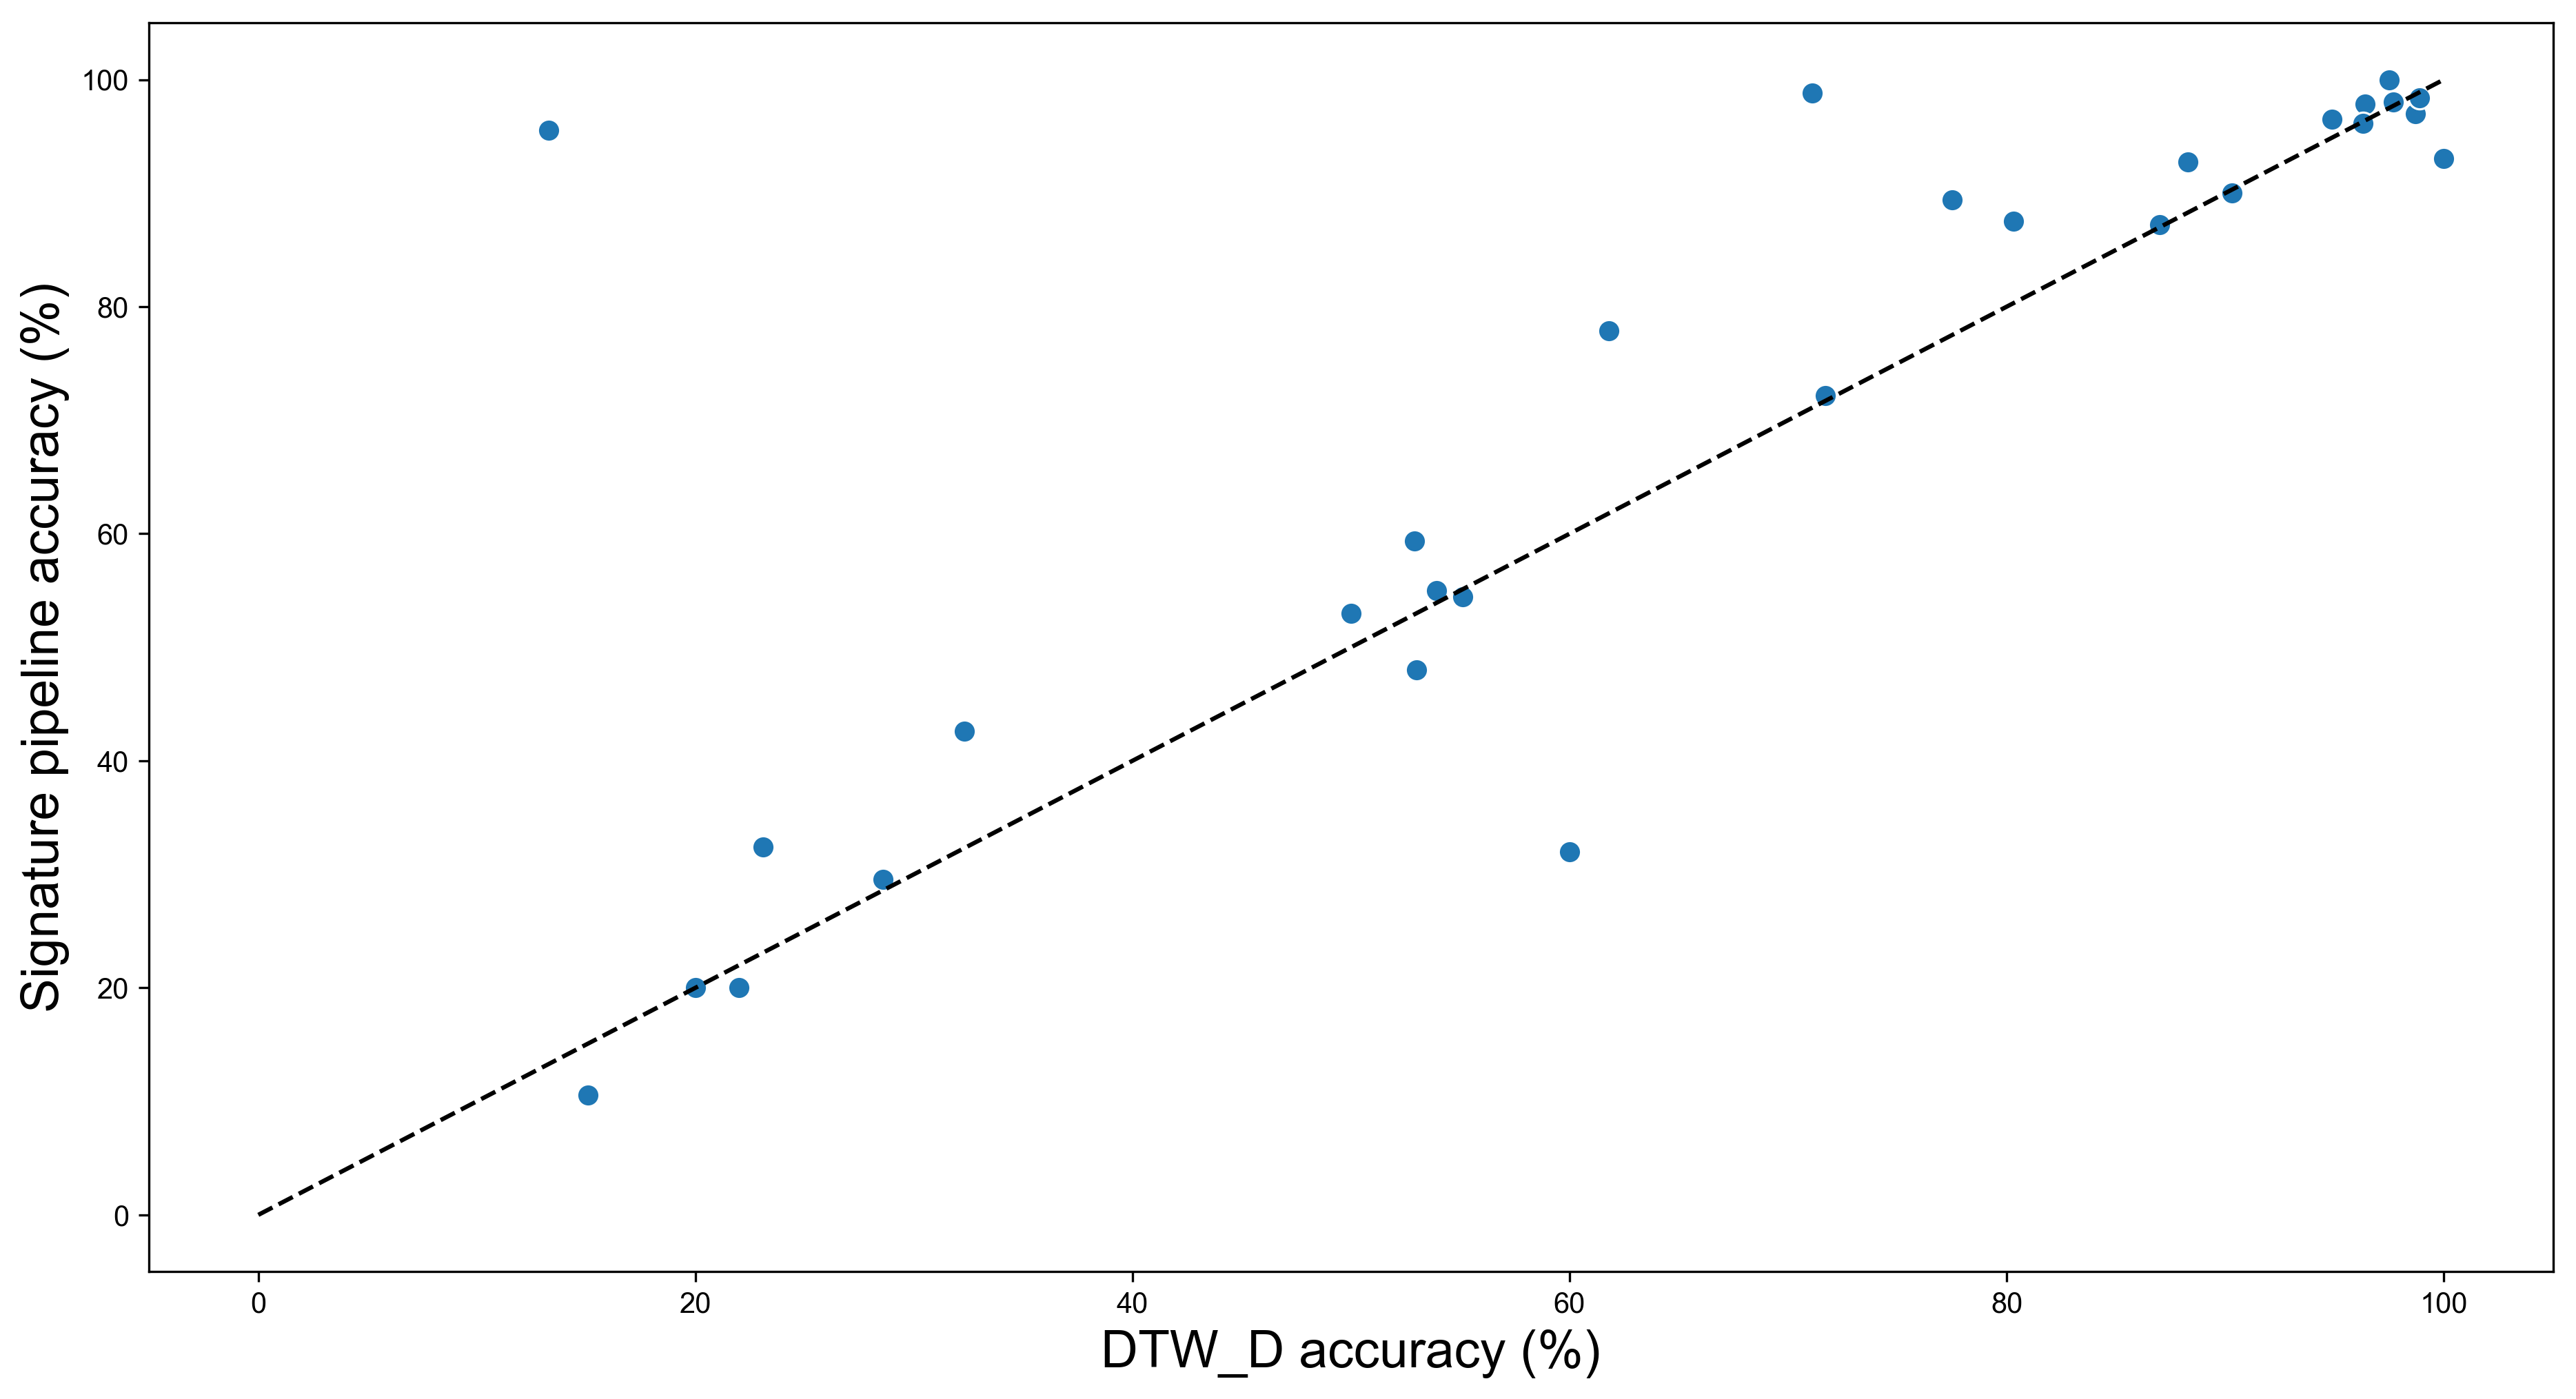
\includegraphics[width=\linewidth]{./images/sig_vs_nextbest.png}
  		\caption{Test accuracy of the signature pipeline against DTW$_\text{D}$, the next best performin algorithim. Each point represents a dataset.}
  		\label{fig:dtw_against_sig}
	\end{figure}

	Finally, we give in Table \ref{tab:best_rf_hyperparameters} the hyperparameters that were selected for each dataset in the signature pipeline model.

	\begin{table}[h]
		\small
		\centering
		\caption{Hyperparameters used for each dataset in the signature pipeline model.}
		\label{tab:best_rf_hyperparameters}
        \begin{tabular}{lccccc}
\toprule
{} & \multicolumn{2}{c}{\textbf{Signature hyperparmeters}} & \multicolumn{2}{c}{\textbf{RF hyperparameters}} & \textbf{Other} \\
\cmidrule(lr){2-3} \cmidrule(lr){4-5} \cmidrule(lr){6-6}
\textbf{Dataset} & Depth &  Dyadic depth & Max depth &  Num estimators &  Training time (s) \\
\midrule
ArticularyWordRecognition &     2 &       2 &            45 &               500 &           60.3 \\
AtrialFibrillation        &     1 &       2 &          None &                50 &           35.9 \\
BasicMotions              &     2 &       2 &            24 &               100 &           19.3 \\
CharacterTrajectories     &     4 &       2 &            80 &               500 &          181.4 \\
Cricket                   &     2 &       4 &             6 &               500 &          249.0 \\
DuckDuckGeese             &     1 &       2 &            16 &               100 &          140.9 \\
ERing                     &     2 &       3 &             8 &              1000 &           16.7 \\
EigenWorms                &     3 &       3 &            12 &               100 &          250.1 \\
Epilepsy                  &     2 &       3 &             8 &              1000 &           42.8 \\
EthanolConcentration      &     2 &       4 &            24 &              1000 &          454.2 \\
FaceDetection             &     1 &       4 &             8 &              1000 &         1816.2 \\
FingerMovements           &     1 &       2 &             4 &               100 &           30.8 \\
HandMovementDirection     &     2 &       2 &          None &                50 &           66.3 \\
Handwriting               &     6 &       2 &            32 &              1000 &          280.3 \\
Heartbeat                 &     1 &       4 &          None &                50 &           45.1 \\
InsectWingbeat            &     1 &       3 &            45 &              1000 &         5367.5 \\
JapaneseVowels            &     2 &       3 &             6 &              1000 &           95.4 \\
LSST                      &     4 &       2 &            60 &              1000 &         1590.5 \\
Libras                    &     6 &       2 &          None &               100 &           28.4 \\
MotorImagery              &     1 &       3 &            24 &                50 &          347.1 \\
NATOPS                    &     2 &       3 &            32 &              1000 &           37.8 \\
PEMS-SF                   &     1 &       3 &            80 &              1000 &          252.3 \\
PenDigits                 &     3 &       2 &            80 &              1000 &          302.3 \\
PhonemeSpectra            &     2 &       4 &            45 &              1000 &         2188.7 \\
RacketSports              &     3 &       2 &          None &               500 &           13.9 \\
SelfRegulationSCP1        &     3 &       2 &          None &               100 &          186.6 \\
SelfRegulationSCP2        &     3 &       2 &             6 &                50 &          138.1 \\
SpokenArabicDigits        &     2 &       3 &            45 &              1000 &         1204.0 \\
StandWalkJump             &     1 &       3 &             2 &                50 &          101.5 \\
UWaveGestureLibrary       &     2 &       2 &            60 &               500 &           21.8 \\
\bottomrule
\end{tabular}

	\end{table}



\end{document}